\chapter{Transformer Architectures and LLMs}\label{ch_transformers}
\chapterauthor{Jeff Yoshimi, Pierre Beckmann, Polyphony Bruna, Tim Meyer}{.4, .3, .15, .15}

% Other general sources Helpful annotated python implementation:
% https://nlp.seas.harvard.edu/2018/04/03/attention.html Excellent walkthrough:
% https://e2eml.school/transformers.html Eric T suggests this workshop:
% https://www.youtube.com/watch?v=quh7z1q7-uc

% There are plans to clarify the definition of generalization, discuss
% different types of generalization failure (misclassification, high regression
% error on novel inputs, etc., which then produce many kinds of errors in
% production AI, from bad translations to mis-pronunciation to misunderstanding
% queries), and then within these hallucinations as a type (perhaps: LLM
% outputs that are convincing but factually incorrect).

% Link to Simbrain demo somehow

As discussed in the history section \extref{age_generative_ai}, we have entered
a new stage in the history of neural networks, what we are calling the ``age of
generative AI'', which should be familiar to you via such tools as ChatGPT. In
their most familiar form, a \glossary{large language model} (LLM) based on the
\glossary{transformer architecture} generates text responses to text inputs by
repeatedly predicting the next word or token in a sequence.\footnote{The
concept of token is introduced in chapter \extref{ch_word_embeddings}.
Following practice introduced there we will vacillate between ``token'', which
is more accurate (since it encompasses punctuation, word parts, and other
non-word entities) and ``word'', which is more intuitive.} They are trained on
large datasets of everyday text, like text from the internet, which is easily
available. As noted in section \extref{age_generative_ai}, it is common to
equate ``transformer'' with ``LLM'', but the two concepts are distinct. The
transformer is the neural network architecture, while an LLM is just any model
of language generation that is based on a large dataset. An LLM can be built
out of something besides a transformer, and transformers can be used on things
besides language. For example, some state-of-the-art image classification
models are now transformer-based, and OpenAI has released an impressive video
generation model---Sora, which also runs on a transformer architecture.
However, in this chapter we focus on transformer-based models of text
generation like GPT.\footnote{There are many other models in this class. As of
this writing (June 2024), this includes the OpenAI GPT series: GPT, GPT-2,
GPT-3, GPT-4, and GPT-4o. It also includes BERT (Google's first LLM, which is
now outdated), Gemini (Bard), several Claude models (Anthropic;  semi
open-source), Llama, LLama2 and LLama3 (Meta), and Alpaca (Stanford; open
source). Most of these models can only be accessed online but some can be
downloaded and run locally, further fine-tuned, etc. A list of LLMs ranked by
how well they chat is here: \url{https://chat.lmsys.org/?leaderboard}.} We will
sometimes refer simply to ``LLMs'' by which we mean transformer-based
LLMs.\footnote{There are numerous high quality online resources for learning
about LLMs. An excellent visual introduction is at this website:
\url{https://poloclub.github.io/transformer-explainer/}. 3Blue1Brown is always
excellent on visual intuition and he has a
\href{https://www.youtube.com/watch?v=wjZofJX0v4M&list=PLZHQObOWTQDNU6R1_67000Dx_ZCJB-3pi}{\underline{YouTube
video}}. For a more technical walk through on building an LLM from scratch see
\href{https://www.youtube.com/watch?v=kCc8FmEb1nY}{\underline{Karpathy's
tutorial}}.}
% GPT as a generic term means “Generative Pre-trained Transformer” (though it
% is often also used to refer specifically to OpenAI’s models. Though the
% transformer architecture can be used in many ways, it became prominent
% through its use to support large language models (LLMs), which are language
% models that generate human readable text.}.  Forward ref to pretraining vs
% fine tuning.

%  Like \cite{elhage2021mathematical} say, ``We focus on autoregressive,
% decoder-only transformer language models, such as GPT-3. (The original
% transformer paper had a special encoder-decoder structure to support
% translation, but many modern language models don't include this.) '' Discuss
% topics relating to BERT. (1) Encoders vs. decoders. This terminology likely
% comes from autoencoders, where we compress data down to a latent space and
% then decompress it, capturing essential information and then reconstructing
% it. In the context of transformers, an encoder is responsible for processing
% input sequences to produce meaningful representations (embeddings), which can
% be at the word or sentence level (refer back to the word embedding chapter).
% For example, we can feed a transformer encoder the first halves of hundreds
% of movie scripts and train it to produce the second halves, or we can train
% it to predict the first summary paragraph of a Wikipedia article based on the
% main body of the article. (2) Bidirectional vs. unidirectional is about
% considering the context in both directions during training. BERT considers
% the whole context of a token from both the left and right during training
% while masking specific tokens. This is known as "masked language modeling"
% (MLM) instead of next-word prediction.\footnote{See \cite{devlin2018bert} for
% a detailed explanation.} Instead of modeling language as a left-to-right
% stream of words, where the model predicts the next word based on the previous
% context (as in GPT), BERT masks a token in the middle of the sentence and
% predicts it based on the surrounding context. This has advantages over
% unidirectional left-to-right and concatenated left-to-right and right-to-left
% models since it creates a truly bidirectional representation where the left
% and right contexts are joined together. This approach has, however, faced
% challenges, and for some tasks, left-to-right models like GPT have been found
% to be more effective. I guess it's still used for some purposes but I'm not
% sure. Also, I suppose it's not a realistic model of actual production, though
% perhaps it is a good model of how we represent sentences encoded in memory. A
% relatively clear way to discuss this is as (1) decoder only (GPT, our
% emphasis), (2) encoder only (BERT), and (3) encoder-decoder (text
% translation).  // Encoders essentially act like very powerful, context-aware
% word embeddings—they take an input sequence, process it with self-attention,
% and produce structured contextual representations that can be used for a
% variety of tasks. // The core architecture of encoders and decoders in
% Transformers is nearly identical, with just a few key differences in masking
% and usage. Of course encoder-decoder has cross-attention

% Add LM vs LLM (and also TLM). On LM see Bender, ``we understand the term
% language model (LM) to refer to systems which are trained on string
% prediction tasks: that is, predicting the likelihood of a token (character,
% word or string) given either its preceding context or (in bidirectional and
% masked LMs) its surrounding context.'' So large that Bender et al. call it
% ``unfathomable training data'' ``We take the term _language model_ to refer
% to any system trained only on the task of string prediction, whether it
% operates over characters, words or sentences, and sequentially or not.''
% (Bender)

Earlier efforts at text generation and natural language processing used
supervised recurrent networks (chapter \extref{ch_supervised_recurrent}), which
are limited in various ways, as we saw. In particular, they can only process a
small amount of context, and suffer from the vanishing gradient problem. The
transformer architecture is basically a complex feed-forward network that can
be ``aware'' of multiple kinds of relationships between arbitrarily far-flung
parts of an input stream. Because it is a feed-forward network, many of the
older techniques covered in this book can be applied to the architecture. In
particular, all the lessons of the deep learning revolution (section
\extref{deep_revolution}) apply here, and indeed, transformers are many-layered
deep networks (chapter \extref{ch_cnn}) that make good use of both
\glossary{representational width} and \glossary{representational depth}. They
can be trained on large datasets using highly optimized parallel hardware. Like
all the other networks discussed in this book, they are not just useful as
engineered tools, but are highly relevant both to neuroscience and cognitive
science, and seem to develop meaningful internal representations. 

We start with preliminary discussion of how transformer-based LLMs are trained
using widely available text data, and how a special recursive trick can be used
to make a feed-forward network--which only predicts next words--produce
meaningful conversational outputs. We then discuss how the transformer
architecture itself works. Finally, we consider how LLMs are utilized and
evaluated and the relevance of these models to cognitive science, neuroscience
and other areas, and consider the practical features of how they are built.
Throughout our emphasis remains on the relevance of transformers to cognitive
science.

Changes in this area are rapid, and the relevance of these areas to cognitive
science is only now being studied, so updates to this chapter are expected.

\section{In-Context Processing}\label{inContext}

% David: please check this entire section and think about if it's appropriate
% here and how it works in the context of the whole chapter
Thus far in the book we have focused entirely on learning via updates to weight
and biases, learning via incremental updates to the parameters of a neural
network. Indeed the distinction between performance and learning was made
central to the entire book in the introduction (section
\extref{performanceLearning}). LLMs are no exception; they learn via a great
number of computationally expensive updates to their billions or trillions of
parameters, as we are about to see.

However, LLMs have a remarkable feature that sets them apart from other neural
network models: an ability to process a great deal of information ``live'', in
their ``working memory'' as it were, without any updates to their weights. This
is the basis for much of their power. Without learning a single new thing, that
can reason their way through a problem or innovate a new idea. When further
extended with the ability to do things like search the internet (see ``agentic
systems'' in section \ref{transformersInPractice}) or prompted to take down
notes to itself (see ``prompt engineering'' in section
\ref{transformersInPractice}), LLMs can be quite powerful.

The point is often made in terms of terms like ``zero-shot'' or ``few shot''
learning. The word ``learning'' here is a reference to machine learning, where
the goal is to make AI models that can do things like classify faces or
translate languages. Zero-shot learning refers to the ability of transformers
to perform some novel tasks without any training examples at all. Few-shot
learning refers to their ability to perform some novel tasks after seeing just
a few examples of it (sometimes after just a single demonstration). As an
example of zero-shot learning, an LLM can be given an example of a review like
``this electric drill really held its charge'' and asked if it is positive or
negative, even though it is not a trained model of sentiment analysis. As an
example of few shot learning, an LLM can be given a few examples of a new type
of character in a game and asked to classify a few new ones. It can do this
even though none of its weight or biases is updated! This is quite powerful and
noteworthy. Indeed, the original GPT-3 paper was explicitly titled ``Language
Models are Few-Shot Learners.''

Broadly speaking, this is referred to as \glossary{in-context learning}, though
perhaps ``in-context processing'' is a better description for it. Even if in AI
terms this is learning, in another sense it more resembles the human ability to
process fresh information held in working or short-term memory. The working
memory capacity of frontier LLMs is much larger than that of humans, and they
don't seem to be restricted to juggling the classic 5 $\pm$ 2
items.\footnote{Of note is the discovery that merely giving an LLM a larger
context window does not automatically give it a correspondingly large working
memory. Though some frontier models can hold entire books inside their context,
their attention is spread thin over such a large context and their ability to
successfully cite information will not work as well as it does in a more
reasonably sized context.}
% Some have said that LLMs have anterograde amnesia.  See Karpathy Reference
% back to old NN's not being able to do one-shot learning (and the use of that
% term in psychology).  Also working memory, and framing effects, and how the
% way you currently think of something separately from your existing conceptual
% apparatus can impact your behaviors.

This is a brand new capability of neural networks that has only just begun to
be explored, especially as it relates to cognitive science. Having said that,
traditional parameter-based learning is still the basis of much of the power of
LLMs, and so we turn to that now.

\section{Learning to Speak Internetese}\label{internetese}

In section \extref{languageModelsRecurrent}, we saw how recurrent neural
networks trained on example text can learn to speak in a way that reflects the
statistical properties of the training data. A network trained on Shakespeare
will start to speak fake Shakespeare, a network trained on real math can
generate fake math, etc. Large language models using transformers do the same
thing--they just do it much better. The architecture is better suited to the
task, as we will see, and they can be efficiently trained on far larger
datasets (hence ``large'' being added on to ``language model''). In fact, the
training set for GPT-3 was not all of Shakespeare, or just a bunch of math
papers, but rather a large subset of the \emph{entire internet}, which included
all of Wikipedia, a few compilations of books, and a web-scraped archive of the
internet called ``Common Crawl''
(\url{https://en.wikipedia.org/wiki/Common_Crawl}). See figure
\ref{gptDatasets}. Similar datasets are used to train frontier LLMs. If you've
ever written anything online, there is a decent chance it is part of the
training data of one of those models.

Since all of Shakespeare is on the internet, as well as discussions of every
topic of human endeavor from physics to history, plus plenty of gossip and
random content about popular culture and everything else, these models can talk
about all of these things. They can statistically generalize from that training
data, which consists of a large part of the internet, which in turn encompasses
many of the books and much of human recorded knowledge. In a sense, after an
extensive period practicing, these models successfully speak ``internetese''.

\begin{figure}[ht]
\centering
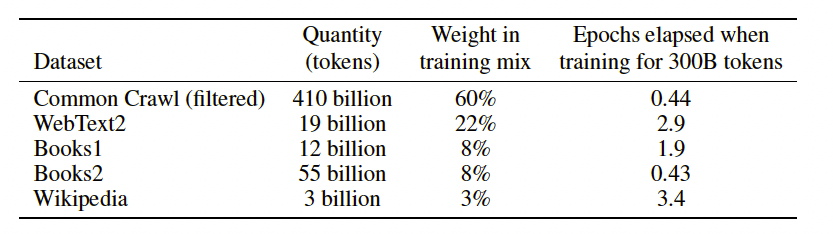
\includegraphics[scale=.4]{./images/gptDatasets}
\caption[From \cite{brown2020language}.]{The datasets used to train GPT-3.
These mostly consist of data scraped from the internet, including all of
Wikipedia, though lots of scanned books are also included.}
\label{gptDatasets}
\end{figure}

The results are impressive. The text frontier models produce is no longer
obviously fake in the way the examples from section
\extref{languageModelsRecurrent} were. In some cases these models arguably pass
the \glossary{Turing Test}, a long-standing test for artificial general
intelligence: over text chat, some models can pass for human to a human
questioner. Whether LLMs truly pass the Turing Test is a matter of ongoing
controversy; we discuss this further in section \ref{llmPhilosophy}.

\section{Training Using Next-Word Prediction}

Recall from chapter \extref{ch_data_science} that a labeled dataset consists of
inputs and targets. As noted there, this kind of labeled data can be hard to
obtain. We might have lots of pictures of people but not know their names or
identities, or have lots of pictures of cats and dogs but not have labeled
whether a given picture is of a cat or a dog. Creating those target labels by
hand for a large dataset is labor-intensive, as it requires humans to manually
look over each picture.

% David the material below was updated based on your comments. Need a bit more
% fanfare on the embedding step, since it is the first step in the pipeline,
% but not sure the best way to integrate it into the discussion Add glossary
% item for auto-regression Tim feedback: currently the discussion makes it
% sound like a random sequence is extracted from a training text. However we
% window across and then use the "Christmas tree" method. This needs to be made
% clear. An image could be used to clarify. In the UC Merced quote can draw a
% window of length context size and then show several steps of it moving.
% Perhaps link to a page showing the full set of training samples and a few
% parameters what the full number would be, and say the formula for how many
% samples we'd get.
LLMs like GPT use a special method (known as \glossary{auto-regression}) to
take \emph{any passage of text} and convert it into a labeled data set that can
be used to train a neural network. The trick is, roughly, to treat the vector
embeddings of a sequence of text tokens (minus the last token in the sequence)
as one big input, and then to treat the vector embedding of the final token in
the sequence as a target. This is called \glossary{self-supervised learning}.
We are still using supervised learning, as in chapter \extref{ch_supervised},
associating inputs with targets or labels, but the targets are not provided
separately and are instead right there in the training data. It's extremely
convenient! Self-supervised training can be used to generate a labeled dataset
from any text document. We no longer have the difficulty of creating
``ground-truth'' labels, as the term ``supervised learning'' may imply. In
practice it's much more like an unsupervised algorithm, in that all we need in
order to train the model is a bunch of text.

For example, consider this block of text adapted from the Wikipedia page for UC
Merced:

\begin{quote}
The University of California, Merced is a public land-grant research university
in Merced, California. It is one of the ten campuses in the University of
California (UC) system. Established in 2005, Merced is the newest campus within
the UC system.
\end{quote}

From this excerpt, we create a bunch of training examples, a list of
input/target pairings. The first pairing we make is the empty input and the
target token ``The''. The next pairing after that is ``The'', target,
``University''. After that, ``The University'', target, ``of''. And so on. By
treating each token as a target for all of the earlier text, every single token
can be made into its own training datapoint.

Technically, the transformer itself does not directly input or output text
tokens. Each token in the input is first turned into a vector using a word
embedding matrix (chapter \extref{ch_word_embeddings}). The target is also
vector encoded, but as an output instead of as an input: the target becomes a
one-hot encoding vector over all possible tokens, where all entries in the
vector are 0 except for the actual next token's entry, which is 1. (We discuss
this further in section \ref{llmOutput}.) In this way we process text into a
table of input-target \emph{vector} pairs, which we can use to train a
feed-forward neural network (see figure
\ref{nextWordPrediction}).\footnote{Note that a longer word like ``university''
would normally be broken up into multiple tokens: \code{un} and \code{iversity}
is a typical tokenization for it, e.g. We are neglecting this complication here
to keep things simple. More on tokenization in chapter
\extref{ch_word_embeddings}.} This table is a matrix where each row corresponds
to the token embedding for one token; it has the shape (sequence size,
embedding dimension) and it is the actual input to the neural network. So
unlike earlier, simpler neural networks, which transformed vectors to vectors
via weight matrices, here we are transforming \emph{stacks} of vectors by
matrices.\footnote{What is actually fed to the transformer is a batch of these
token embedding matrixes, that is a rank-3 tensor with shape (batch size,
sequence size, embedding dimension); see section \extref{sect_tensors}).}
Figure \ref{sequenceDim} illustrates the idea, and introduces some
useful terminology.

\begin{figure}[ht]
\centering
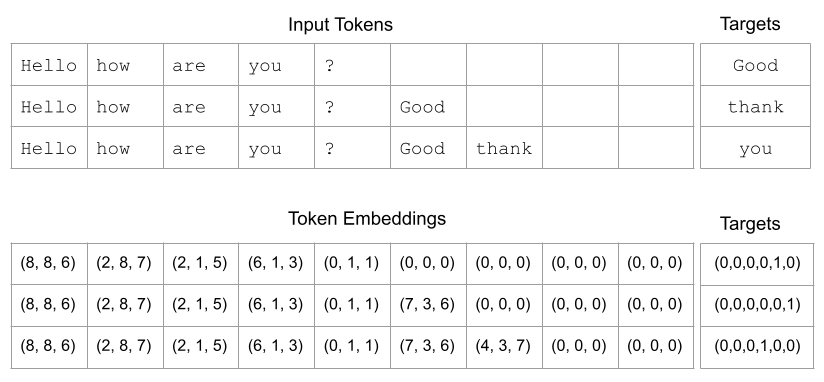
\includegraphics[scale=.45]{./images/contextWindow.png}
\caption[Jeff Yoshimi]{How text sequences can be converted into training
datasets using the method of auto-regression. A set of tokens is converted into
vectors using a token embedding (the vectors shown are arbitrary, just to
illustrate the idea); by concatenating these vectors we get an input vector.
The next token in the sequence is encoded as a target using a one-hot encoding
over all tokens (in this case there are seven possible tokens: six words and
the question mark).}
\label{nextWordPrediction}
\end{figure}

Note that the word embeddings in figure \ref{nextWordPrediction} and figure
\ref{sequenceDim} are 4-dimensional (each token is associated with an array of
4 numbers, a vector in a 4d space). In real LLMs, this ``embedding dimension''
is quite a bit larger--over 12,000 for GPT-3 (see figure \ref{gptParams}).

\begin{figure}[ht]
\centering
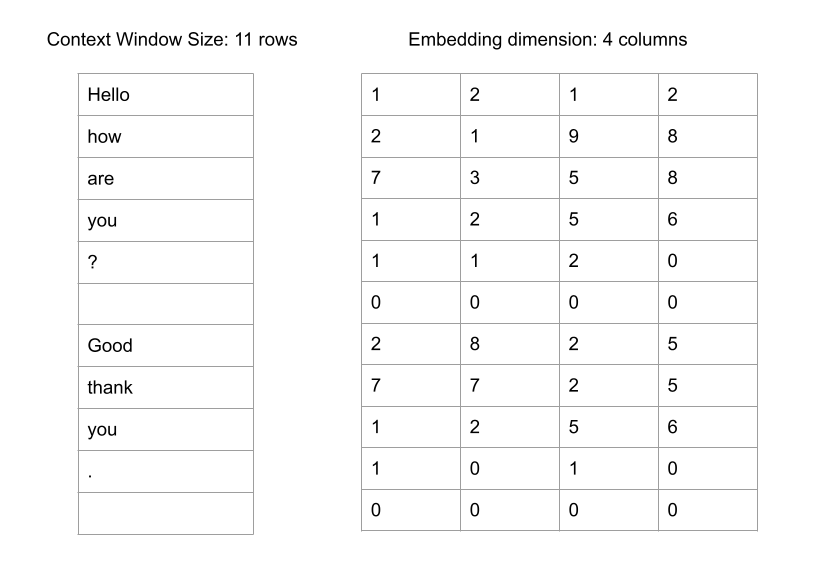
\includegraphics[scale=.45]{./images/contextWindowAsStack.png}
\caption[Jeff Yoshimi]{The context is associated with a matrix that can
be thought of as a stack of vectors, one for each token. Notice that ``you''
occurs twice and is associated with the same vector.
}
\label{sequenceDim}
\end{figure}

There is a key conceptual takeaway from all of this, central to understanding
LLMs. We can think about a context as a stack of tokens converted into a stack
of vectors, where the vectors correspond to embeddings of the tokens in a
vector space. The context then gets transformed as it travels through the
network, ultimately becoming next-token predictions. Thus the repeated ``you''
will change its representation as it is processed. This may seem confusing at
first; don't the numbers get all jumbled up when we matrix multiply? But recall
the discussion of matrix multiplication and the ``row processing'' perspective
(section \extref{matrixMultiplication}), where we can view think of a matrix
multiplication as taking a stack of $N$ row vectors on the left, multiplying
them by a matrix produces on the right, to produce another stack of $N$ row
vectors, each of which has been \emph{separately processed} by the matrix on
the right. As a result, we can separately track the transformations a token's
vector representation goes through as it makes its way through a network.  We
will circle back to this idea below when we discuss the ``residual stream''.

% We can picture the residual stream as a big shared whiteboard that every
% head can read from and write to.

% \footnote{This idea is illustrated in section \extref{wordEmbeddingMatrix},
% where it was described as a ``token embedding matrix''.}

% Tim feedback: positional feedback happens too fast.  A mystery is thrown at
% the reader. Take time and unpack. To make it clear concretely what happens,
% see the picture I made (positionalEncoding.png). Clarify position is position
% in sequence.  But it's also confusing how this doesn't mess up the semantics
% of say king - queen  = man - woman.  The response is something like we now
% have slightly enriched semantics, like king-at-start-of-sequence, etc., and
% noting that gradient descent will discover the same things it did before,
% PLUS representations that are sensitive to position. Separate question: why
% aren't the weights enough to provide positional encodings, since there is
% some implicit ordering in it. Another option for positional encoding is to
% just leave it out from the discussion One interesting feature of transformers
% is that they do not inherently know about the order of tokens in a sequence.
% Thus, the tokens in a token embedding matrix are in a sense unordered (their
% position in a stack is an order, but this information is not easily available
% to the network given how it processes information), which allows for
% super-fast parallel processing. Thus a \glossary{positional embedding} (or
% ``positional encoding'') is used to modify the vectors in a token embedding
% matrix, often by using a trigonometric function (like sine or cosine) that
% simply adds more or less to the numbers in the vectors depending on where
% they are in a sequence.\footnote{This is a kind of feature engineering trick;
% see chapter \extref{ch_data_science}.}  %In figure
% \ref{transformerBlockSimple} the encoding subtracts 1 from each component of
% the word embedding for ``Hello'' (which was $(8,8,6,1)$ for the sample
% embedding in figure \ref{nextWordPrediction}).
  
\section{How Conversations are Generated from a Feed-Forward
Network}\label{recursiveTrick}

% Pictures needed for recursion trick and context window. E.g take second
% figure in this chapter and add some arrows or numbers showing how to generate
% sequences. Clarify somewehere that padding is not usually used at the end of
% a context window. The stacks of vectors and self-attention matrix can be
% variable-sized depending on the length of the current chat. This is missing.

One confusing thing about figure \ref{nextWordPrediction} is that we go from a
large input covering a whole set of tokens to a single token as output. So
great, we can predict single words. But how do we go from single words to
generating long text outputs, or having conversations? In fact, in hearing
about generative AI as ``next word prediction'' machines, you may have
sometimes wondered how such complicated things can happen when all these models
do is predict next words.

% More discussion of special tokens like end-of-sequence is probably needed,
% and maybe further up. The network itself is feedforward, but its interaction
% with an environment is recursive.
The answer is by using what we can call the ``recursive trick''. This trick
allows us to take a feed-forward network that only predicts next words and use
it to produce streams of text output. In fact, it's remarkably simple. We feed
a network a set of inputs corresponding to string of text, and it produces an
output corresponding to the predicted next token. That output is then appended
to the previous input, and this longer input is now fed back to the network.
This process is repeated to produce a stream of text outputs. This technique
can be used to generate unending sequences of text from any
prompt.\footnote{Notice that this is a kind of recurrence, and arguably this
makes LLMs used in this way a kind of recurrent network. Outputs are fed back
in as part of inputs. However, the outputs are text that must be converted back
to text inputs, which are then vector encoded. In fact, recurrent networks were
originally used for text processing, as we saw in chapter
\extref{ch_supervised_recurrent}, but it turns out that fancy feedforward
networks used in this way outperform them. (In those cases, a vector
representation of each token in the sequence would be presented separately:
``hello'', ``how'', ``are'', ``you'', ``?'').} The prompt is our input, and
then answers are generated using the recursion trick. Text will continue to be
generated until a special end-of-sequence token is reached.\footnote{For more
on the post-training that enables ChatGPT and other frontier models to carry on
a conversation with a human-like persona, see \extref{ch_value_alignment}.}
% David: the footnote above should be changed to a forward reference to the new
% chapter Also RLAIF — Reinforcement Learning from AI Feedback

So this gets us one response. But then you type a new question. That
\emph{entire question} is appended to the \emph{entire past conversation}
including both what you and GPT have said so far.

Suppose, for example, we want to ask a network ``hello how are you?'' The input
to the network is the whole sentence $\{$``hello'', ``how'', ``are'', ``you'',
``?''$\}$. Let's  not worry about the vector embeddings, and just see the
general idea, as shown in figure \ref{gptRecursedInputs}. Notice that the
initial prompt is the initial input, but then the prompt \emph{and} the first
word of the response are used as the next input, and this process can be
repeated until a response is written out.
  
\begin{figure}[ht]
\centering
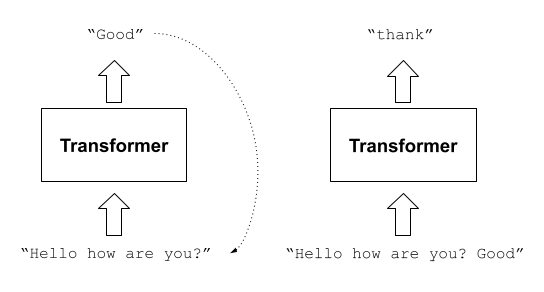
\includegraphics[scale=.7]{./images/gptRecursedInputs.png}
\caption[Jeff Yoshimi]{A schematic view of how ``conversations'' are generated
from feed-forward networks in systems like ChatGPT. The output at one time is
concatenated to the input at that time, and that is then used as the input at
the next time step. This process is repeated to generate a full response.
}
\label{gptRecursedInputs}
\end{figure}

Of course, as we keep doing this, the inputs to the network get larger and
larger--there must be some limit to how far we can go, right? The answer is
yes. An LLM's hyperparameters include a \glossary{context window} value: the
maximum length of context that the LLM will read. At the start of a chat
instance, the context starts small, with only an initial prompt. In a dialog,
the prompts from a person and the responses from the LLM are both included
until the context window is filled. Thus, if the context window is large
enough, whole series of back and forth conversations can be processed. All the
prompts and responses up until the current point are part of the input, and
then the LLM uses the recursion trick to generate new responses that are
sensitive to everything that's been discussed thus far. When the length of the
context grows larger than the context window value, text is simply dropped from
the start of the context, to fit (from a computer science standpoint, this is a
queue). This is intuitive in figures \ref{nextWordPrediction} and
\ref{gptRecursedInputs}. These context window values can be remarkably large.
GPT-3 has a context window of about 2,000 tokens or about 6 pages of text, and
early versions of GPT-4 had context windows of 32,000 tokens or about 72 pages
of text.

\begin{figure}[ht]
\centering
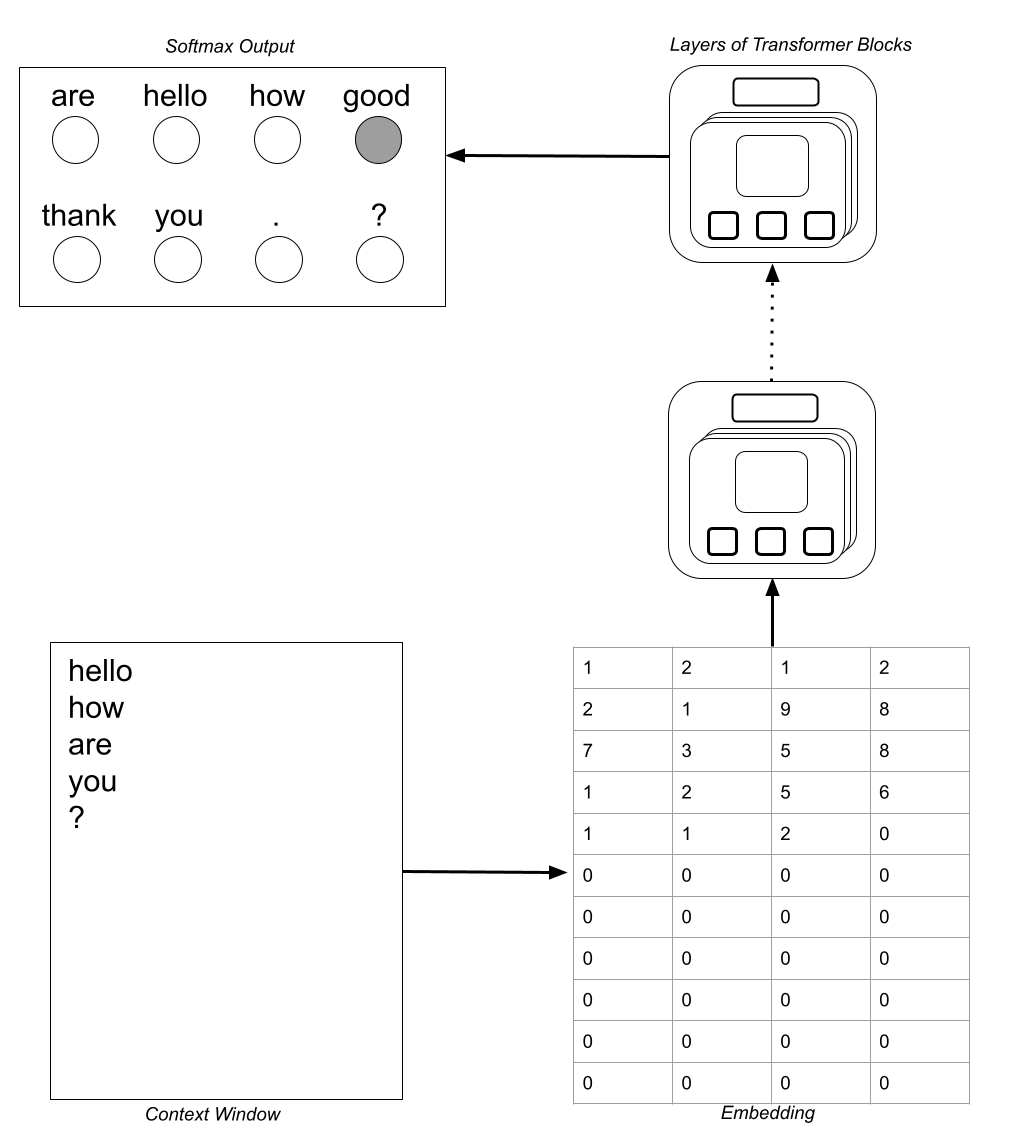
\includegraphics[scale=.2]{./images/TransformerOverview.png} \; \; \; 
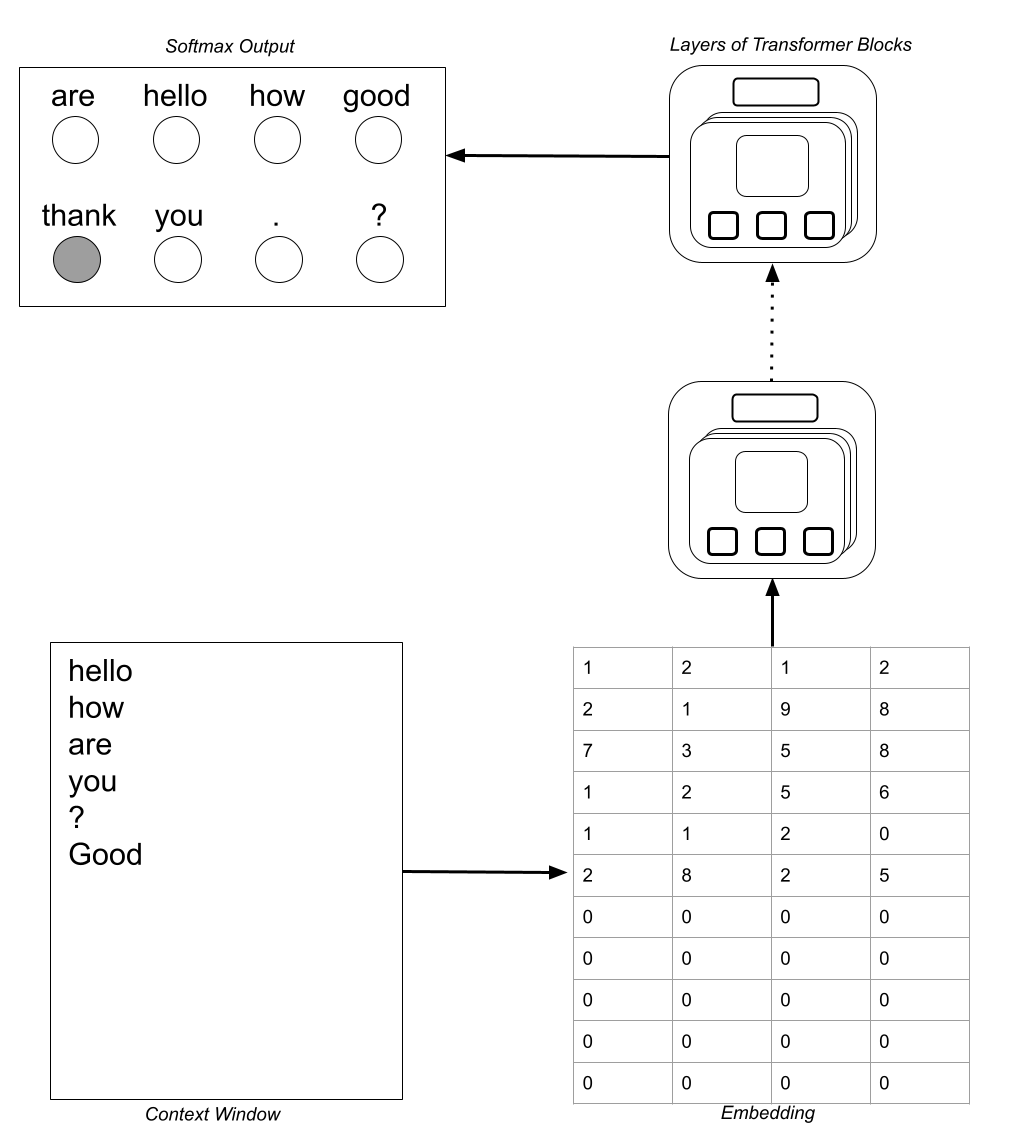
\includegraphics[scale=.2]{./images/TransformerOverview2.png}
\caption[Jeff Yoshimi]{A first look at the process of a conversation unfolding
through a network, showing the stack of word embeddings associated with the
context, the transformer blocks, and the softmax output. Note that the
most active output is associated with a token that is added to the context
window on the next time step. Shown are two time steps. On the left the network
has output a response of ``Good'' in response to the query, and that output is
placed in the context using the recursion trick.
}
\label{transformerOverview}
\end{figure}

\section{The Transformer Architecture}\label{transformers}

% \footnote{Two excellent visualizations are \url{https://bbycroft.net/llm} and
% \url{https://poloclub.github.io/transformer-explainer/}.}
 
We have thus far covered high-level features of how LLMs work, but have treated
the transformer as a black box. The time has come to open up the box. How does
the fancy feed-forward network at the heart of these models work? Its power
rests on a few novel architectural innovations, which combine representational
width and representational depth with a special form of context awareness. All
the things we've seen about other neural networks still apply here. The
transformer is a kind of deep feed-forward network, which uses a huge amount of
training data. But the key innovation is that, within each ``layer'', the
transformer can develop many forms of context representation which relate all
the tokens in a context to each other.

\subsection{Blocks}

The transformer architecture \cite{vaswani2017attention} is made up of layers
or ``blocks'', which are specialized to process the large contexts that are fed
into the network as input. With training, these blocks learn to find long-range
dependencies between different parts of a context. Recall that the context
includes an original prompt, its own response to that prompt, etc.; it includes
the \emph{entire exchange} you've had with GPT up to the current point, so long
as it fits in the context window. Each block combines an attention head and a
standard feed-forward network or MLP (see figure \ref{transformerBlockSimple}).
We maintain the ``row processing'' perspective of section
\extref{matrixMultiplication} throughout the discussion. That is, we forget
about batch processing, and focus on a stack of vectors, each corresponding to
one token in the context. This stack is first processed through the attention
heads, and then through the MLP.

% More on normalization, "scaled dot product"
The attention head is where the contextual awareness occurs. Each token
representation in the entire stack is compared to every other one. In our
simple example, ``hello'' is compared to ``how'', ``are'',  ``you'', and also
to itself. These comparisons occur using three matrices: $\textbf{K}$,
$\textbf{Q}$, and $\textbf{V}$, which stand for key, query, and value. First
the input to the block, a stack of vectors representing tokens, is multiplied
by the key and query matrices to produce two new stacks of vectors. These
stacks of keys and queries are then multiplied (using a dot product) in all
possible combinations and then normalized to produce a context representation
(see the discussion of vector comparisons and vector comparison matrices in
section \extref{vector_comparisons}). We can think about this as a kind of
table lookup, where the query asks a kind of question, and the key is a
potential answer\footnote{For thinking about the key and query vectors,
$\textbf{K}$ and $\textbf{Q}$, see
\url{https://e2eml.school/transformers.html}, which develops the idea that keys
and queries are being used in a table lookup procedures, as the terms suggest.
The queries are source terms, the keys target terms. The key scans across
past-tokens (due to the triangular mask that is used) and selects information
useful for predicting.} The resulting matrix reflects the degree to which the
different token representations are facing in the same or different directions
in the embedding space. These entries also called self-attention scores. For
example, in the sentence ``I went to the bank'', there will be a score for bank
in relation to ``the'', "to'', etc.\footnote{Only backwards relationships are
examined, a ``triangular mask'' is applied to the matrix to 0 out the upper
triangular, so that token representations are \emph{not} compared to future
tokens because that would make the word prediction task too easy. This is
visible in the Simbrain representation.} This self-attention matrix is then
itself used to process the stack of vectors produced by multiplying the inputs
by the value matrix $\textbf{V}$.\footnote{For thinking about the value vector
$\textbf{V}$, see Tom Yeh's
\url{https://www.byhand.ai/p/8-can-you-calculate-a-transformer}, which focuses
on the attention matrix and the "attention weighted features" that occur when
activations are passed through it (that is, the output of the attention head).}
In this last step all the token representations are enriched by contextual
information. So the output of the attention head is a stack of token
representations that reflects dependencies between them. All tokens, no matter
how far apart they are within the context window, can still influence each
other. The self-attention mechanism learns what relations between words in a
context window are important; in a sense it learns what to focus on (hence
``self attention'').

% David. Thoughts on how much of these comments to add and how? Residual
% connections are also used. That is, the input to the block is added directly
% to the output of the multi-head attention mechanism. This allows the gradient
% descent algorithm to have a direct route backwards through the blocks of the
% network, as a way to address the vanishing gradient problem (see chapter
% \extref{ch_supervised_recurrent}). } Attention heads can be understood as
% independent operations, each outputting a result which is added into the
% residual stream. Attention heads are often described in an alternate
% “concatenate and multiply” formulation for computational efficiency, but this
% is mathematically equivalent. Attention heads can be understood as having two
% largely independent computations: a QK (“query-key”) circuit which computes
% the attention pattern, and an OV (“output-value”) circuit which computes how
% each token affects the output if attended to. > YES! [KQV] are intermediate
% results in the computation of the low-rank matrices [i.e projections to lower
% dimensions that remove noise and distll out something essential]. It can be
% useful to describe transformers without reference to them [so ignore them?]
% Composition of attention heads greatly increases the expressivity of
% transformers. There are three different ways attention heads can compose,
% corresponding to keys, queries, and values. Key and query composition are
% very different from value composition. > YES and cf "representational depth"
% All components of a transformer (the token embedding, attention heads, MLP
% layers, and unembedding) communicate with each other by reading and writing
% to different subspaces of the residual stream. Rather than analyze the
% residual stream vectors, it can be helpful to decompose the residual stream
% into all these different communication channels, corresponding to paths
% through the model. > \cite{elhage2021mathematical}

\begin{figure}[ht]
\centering
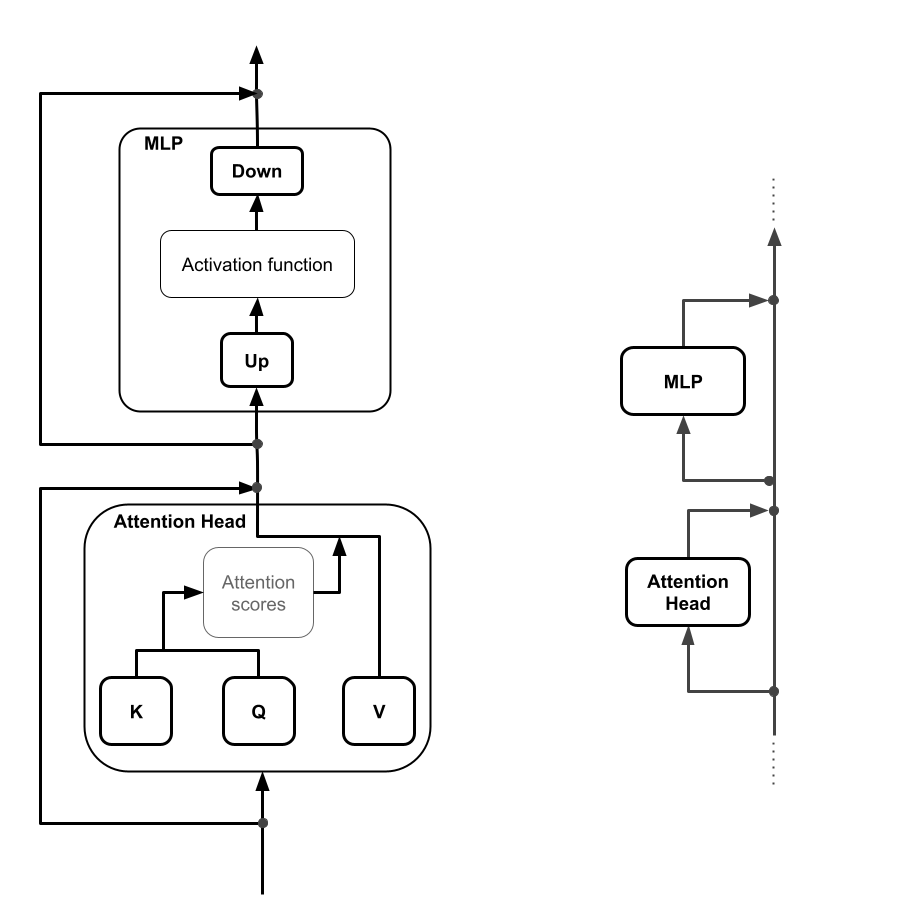
\includegraphics[scale=.3]{./images/transformerBlockResidualStream.png}
\caption[Jeff Yoshimi with consultation from Tim Meyer.]{(Left) One transformer
block, with a single head. The matrix  (or tensor) of activations being fed to
the block is processed by three matrices: $\textbf{K}$, $\textbf{Q}$, and
$\textbf{V}$.  Generally speaking these are down projections that reduce the
size of the data.  $\textbf{K}$ and $\textbf{Q}$ are used to generate a
self-attention matrix. The input to the block is processed through $\textbf{V}$
and then through the self-attention matrix, and then through an up projection
(not shown) so it is back to the same size as the input. After leaving
attention, there is a skip projection from the input and the resulting
activations are passed into a standard feed-forward network or ``MLP''. The MLP
typically involves a hidden layer that is larger than the input (hence up
projection and down projection). From the input to the output of the MLP there
is another skip connection. (Right) It can be helpful to foreground the skip
(or residual) connections rather than the sublayers themselves, seeing the
original embeddings as traveling straight down the length of the network, with
attention and MLP sublayers reading from and then writing to this ``residual
stream''. Note that the left and right diagrams present the same computational
structure, just with a change in their point of emphasis. Bolded elements in
the diagrams are made out of trainable parameters.}
\label{transformerBlockSimple}
\end{figure}
% Include Simbrain screenshot? 

% milliere2024philosophical1 calls this a "residual stream" and refers to a
% "linear map hypothesis". The linear representation hypothesis, according to
% which high-level concepts or features are represented linearly as directions
% in a neural network’s activation space. This hypothesis is often taken to be
% central to the agenda of mechanistic interpretability" (bruck, p. 17)

% Citations and more on what happens in the MLP. The 2/3 weights thing; Pierre
% email
Once processed through the attention mechanism, activations are processed by a
feed-forward network, an MLP, whose hidden layers is typically higher
dimensional than the input.	The MLP plays an important role. It contains more
weights than the rest of the block. It can be helpful to see the transformer
block as basically made up of these two functional pieces, together: the
attention mechanism specializes in identifying long-range dependencies in the
context and upweighting those relationships, while the MLP sublayer can then
perform arbitrary operations on that curated information (such as reciting
relevant facts learned during training, e.g.). Since they are used one after
the other in a transformer block, the transformer's architecture is setting it
up to recall what is relevant and then process that relevant data.

% Add backwards ref to resnet discussion
There are skip (or residual) connections before and after the attention head
and the MLP, and as a result we can think of the transformer block as reading
from and writing to a single \glossary{residual stream} of activations in a
latent space \cite{elhage2021mathematical, milliere2024philosophical2} whose
dimension is the embedding dimension (recall the discussion in section
\extref{flowDiagrams}).\footnote{The concept of a residual is that of an error
in statistics, how far data lies from a regression curve, for example. The idea
here is that rather than transforming information completely from one layer to
the next, that the layers just produce ``deltas'' on a single stream of
information flowing through the stream, they operate on these ``residual''
errors, as it were. The idea originates in deep networks.} This is the
perspective shown in the right panel of \ref{transformerBlockSimple}, and it's
a crucial perspective, because it means that there is a single space we can
focus on. As the stack of token representations moves upwards through the
residual stream, it is progressively further and further enriched with context
information by attention heads and by other learned information or operations
by the MLPs.\footnote{Since we can think of these as reads and writes, this
also means that we can think in a more algorithmic or symbolic way about what
is happening in the network, with representations being shuffled and moved
around and erased, in a nod to the older views of classical AI (we return to
this topic in the discussion of philosophy at the end of this chapter).} Thus
the token representations are continually enriched, growing into the model's
final output from that forward pass. 

That is the basic architecture. We can get a useful lens on its learned
functionality (what it will be able to do after training) with the concepts of
representational width and representational depth.
 
% Eric S: At multiple heads: Can you explain a bit more in ordinary language
% what the functional importance of these transformation is?  Maybe some
% examples would help. What kinds of things generate high vs low
% self-attention?
First, consider representational width, which corresponds here to the fact that
there are multiple attention heads in every attention sublayer: it is a
``multi-head'' attention mechanism. This allows the network to pay attention to
different features of the token representations coming to it through the
residual stream (see figure \ref{multipleHeads}). Each head indpendently
carries out all the attention head operations described above. The
\emph{reason} that $\textbf{K}$, $\textbf{Q}$, and $\textbf{V}$ are typically
down projections, taking the input stream and splitting it up into multiple
smaller attention matrices, is that that allows multi-headed attention to think
about the context in several distinct ways in parallel.\footnote{The
dimensionality of each head is often the embedding dimension divided by the
number of heads, so that when the outputs are concatenated, the original
dimension is restored. In figure \ref{gptParams}, the number of inputs to each
head, $d_\text{head}$, is equal (or almost equal) to the embedding dimension
$d_\text{model}$ divided by the number of heads $n_\text{heads}$.} For example,
if the embedding dimension were 9, it might be projected into three separate
3-dimensional heads.\footnote{Thus, for each head, the $\textbf{K}$,
$\textbf{Q}$, and $\textbf{V}$ matrices would typically have dimensions $3
\times 9$, where 9 corresponds to the input dimension from the previous layer,
and 3 refers to the reduced dimensionality for each head (note that for
efficiency, these matrices are often combined into a single larger matrix.)}
The outputs of all the heads are then up-projected back to the size of the
residual stream and added together. Multi-headed attention, in letting the
network use \emph{multiple} ways to scan over the context for relevance, is a
bit like convolutional networks (section \extref{convolutionalLayer})
developing \emph{multiple} filters to analyze an image (which we also termed
representational width).

% This part is not clear yet. Also, the figure should probably have
% ``de-embedding'' and ``softmax'' in the final layer separate from the FF part
% somehow. Discuss how the input and output sizes stay the same through the
% layers. According to GPT this is for multiple reasons (simple design and
% stacking, facilitate residual connections, stable layer normalization,
% uniform attention mechanism).

\begin{figure}[ht]
\centering
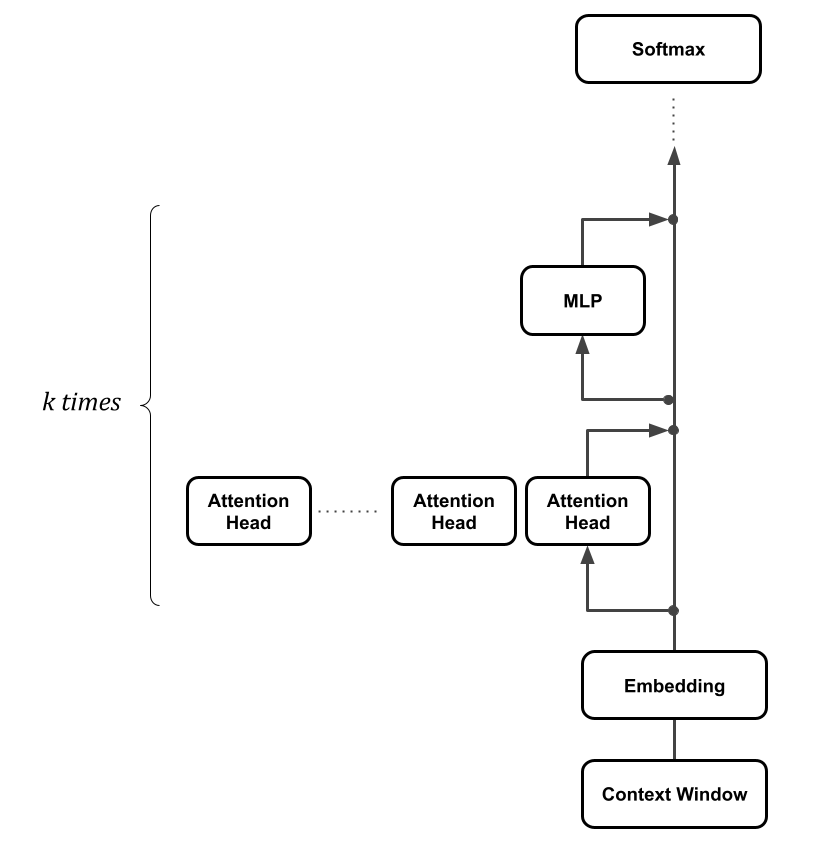
\includegraphics[scale=.35]{./images/transformerBlockMultiHeadResidualStream.png}
\caption[Jeff Yoshimi with consultation from Tim Meyer.]{Schematic of the
transformer architecture. Multiple transformer blocks are stacked, capturing
representational depth, as in a CNN. Each block contains a multi-head attention
mechanism, where each head learns to represent inputs to the block in a
different way, capturing representational width. The outputs of the multiple
heads are combined in a standard feed-forward network. (Some further elements
of the transformer architecture, like LayerNorm, are not shown here.) As with
before, bolded items contain trainable parameters that are updated via gradient
descent.}
\label{multipleHeads}
\end{figure}
 
Now we take a lesson from deep networks, and simply stack many of these
transformer blocks on top of each other ($k$ times in figure
\ref{multipleHeads}) to allow for increasingly sophisticated representations.
This is representational depth; the idea was already hinted at above in the
initial discussion of the residual stream. As token representations move
through the layers of attention heads and MLPs, they acquire more and more
context information and are steadily transformed, with the vectors
corresponding to them in the latent space reoriented in slightly different
directions to reflect this refinement of meaning.\footnote{The 3Blue1Brown
video linked at the start of the chapter has useful visualizations of this
process, represented geometrically.} Recall that with deep networks for vision,
we get features, features of features, features of these features, etc., whose
activations match neural response properties of different layers of the human
visual system. This builds on the old idea of the \emph{Pandemonium} model
(section \extref{cog_rev}), which involved (at successive layers): edge
detectors, detectors for combinations of edges, detectors for combinations of
these combinations (e.g., fragments of letters), and ultimately full letter
detectors. In a similar way, the successive layers of a transformer language
model correspond to increasingly complex features of the input stream,
including syntactic categories, semantic properties, and far more complex
features as well.\footnote{The extent to which activation patterns correspond
to syntactic or semantic features is measured using post-hoc interpretation
techniques such as probing. As with so many other neural network features,
these were not ``programmed in'' by the engineers, but are emergent from the
network after training, and are studied and described by scientists after the
fact.}

% Work with Eric S on integrating this point here. We could say something like,
% this explains a rather striking feature of LLMs: that you can enter prompts
% like ``First, describe X. Next, describe Y. Finally, describe Z'' and it will
% do it. By the time the LLM is describing Z, there might be a hundred or more
% words between "Z" in the prompt and the output concerning Z.  If X and Y have
% little to do with Z, then this is a fairly long gap to cover that cannot
% readily be explained without some way to bridge between the initial Z in the
% prompt and the description of Z in the output."] It would be nice if this
% section could explain a bit more how this architecture enables such
% structured outputs, which one wouldn't expect from say a next-word,
% next-word, next-word autocomplete on your phone. (GPT3 could also do this,
% unreliably, so I think the human feedback training isn't essential to this
% type of task, if I'm recalling correctly that GPT3 was a pure transformer
% without the human feedback training.)

The transformer architecture is trained using gradient descent and supervised
learning (chapter \extref{ch_supervised}). These are the same ideas used for a
simple feed-forward network trained using backprop, but with many more
trainable components. The error signals used in gradient descent are being
back-propagated through a \emph{lot} of stuff here! Residual connections are
especially important in this regard, as they allow gradient to effectively flow
backward through the length of the transformer without disappearing or
exploding in value, even at the earliest layers. Much of the art of
architectural design lies in giving a network both lots of structural latitude
to learn the links it needs to \emph{while also} having an architecture that can
efficiently train at scale.

\subsection{Softmax Outputs}\label{llmOutput}

The first step in a transformer is to embed inputs, as we've seen. The next
step is to transform these inputs using a series of blocks that are wide
(thanks to multiple heads) and deep (thanks to multiple blocks). When all the
processing is done, the last step is to un-embed the outputs, converting
vectors back to tokens. 

In figure \ref{nextWordPrediction} we saw that while inputs use a word
embedding, outputs are probability distributions over the whole vocabulary, and
targets are one-hot encodings consisting of all zeros and a single ``hot''
number (the number 1) corresponding to the predicted next word (on one-hot
encodings, see section \extref{wrangling}). When target data are binary one-hot
encoded labels, the task given a network is a classification task (section
\extref{classificationRegression}). Thus transformers are technically
classifiers, which classify input texts according to what word is likely to
occur next. Classification can here be seen as serving as a \emph{proxy task}.
Our actual task is to predict a set of probabilities over next tokens. The
output of an LLM is a set of probabilities over next tokens.\footnote{The
interesting thing is that by \emph{trying} to perfectly classify next tokens
(an impossible task), we end up with good probabilities, which is exactly we're
after. Here is a way to think of it. If the model was trained to 100\% accuracy
on the classification task, then it would always generate the same sentences
from the same prompts (because it would assign one unique token to the current
input). But then it could not generate new instances of text.}

The output of an LLM is often a \glossary{softmax} layer with around 50,000
outputs, which  indicate how probable all the tokens are given the input (all
the prompts and responses in the context window so far). The softmax
temperature parameter can be used here (see section
\extref{wta_softmax_section}): higher temperatures will make the outputs more
random or ``creative''. See figure \ref{transformerOverview} for how this might
look for our simple example, where the output vocabulary just contains 7
tokens. 

Once we have a probability distribution over tokens, we select one of the most
probable next tokens and that becomes the output. This is usually done by
sampling from among the top $n$ most probable next tokens. Thus the final
softmax layer does the opposite of what the embedding layer does. Rather than
converting from tokens to activations, it converts from activations to tokens,
and is thus a ``de-embedding'' layer.

\subsection{Parameters and Hyperparameters}

By way of summarizing, consider the parameters and  \glossary{hyperparameters}
associated with a transformer-based LLM. Recall that parameters are primarily
weights and biases (i.e values that are updated during training) while
hyper-parameters are values that determine the structure of a network but that
are not updated during training.

Figure \ref{gptParams} shows the  number of parameters for a range of GPT-3
subvarieties as $n_\text{params}$. The released version of GPT-3 had 175
billion weights and biases. By comparison, our xor 2-2-1 network had 3 biases
and 6 weights, or 9 parameters. A standard convolutional neural network might
have millions of parameters. So this is just massively larger. Not
surprisingly, these networks have gotten even larger. GPT-4 has about 1.76
trillion parameters.\footnote{It takes large server banks that  consume huge
amounts of energy to run these models, and so there is a thread of research
attempting to achieve similar performance with smaller models, some of which
can be run on a  personal computer. For example, Gemma2B achieves performance
similar to GPT-3.5 with 2 billion parameter. See
\url{https://developers.googleblog.com/en/smaller-safer-more-transparent-advancing-responsible-ai-with-gemma/}.}
Figure \ref{gptParams} also shows the values of several hyperparameters such as
number of layers ($n_\text{layers}$), corresponding to representational depth,
and number of heads ($n_\text{heads}$), corresponding to representational
width.\footnote{Notice that the size of the heads, $d_\text{head}$ is equal or
almost equal to  $d_\text{model} \times n_\text{heads}$ (some mismatches are
allowed).} The size of the token embedding  $d_\text{model}$ is also shown, as
are the learning rate and batch size. Notice that these are all concepts we
have seen in one way or another (often directly) in earlier chapters. All the
same ideas are being used but on a larger scale.

\begin{figure}[ht]
\centering
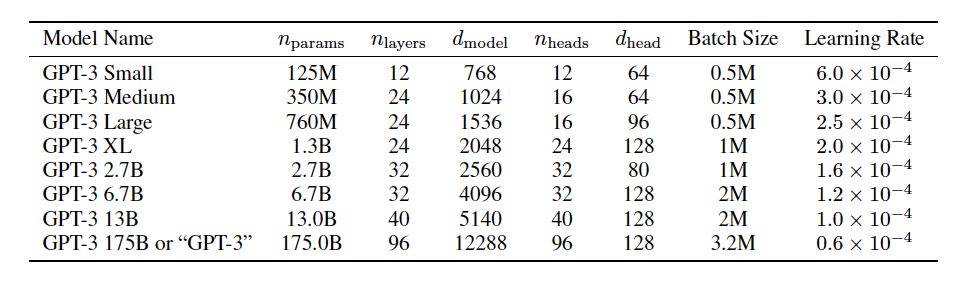
\includegraphics[scale=.4]{./images/gpt3_params.png}
\caption[\url{https://arxiv.org/abs/2005.14165}.]{Number of parameters and
values for some of the hyperparameters used in training different versions of
GPT-3.
}
\label{gptParams}
\end{figure}

The size of the context window is another hyperparameter not shown in the
figure. According to IBM research, ``when ChatGPT made its debut nearly two
years ago, its window maxed out at 4,000 tokens. If your conversation went over
the 3,000-word chat-interface limit, the chatbot was likely to hallucinate and
veer off-topic. Today, the standard is 32,000 tokens, with the industry
shifting to 128,000 tokens, which is about the length of a 250-page book. IBM
just open-sourced on Hugging Face two Granite models with a 128,000-token
window, and more are on their
way.''\footnote{\url{https://research.ibm.com/blog/larger-context-window}.}

\section{LLMs and the Cognitive Sciences}\label{llm_cogsci}

% Add more on Turing Test (or remove the forward reference from the start of
% the chapter)
As with many architectures discussed in this book, transformer-based LLMs are
major objects of scientific interest, even if they were developed for
engineering applications (see chapter \extref{ch_applications}). They are
interesting for the obvious reason that they are in some sense the best
cognitive models ever produced. They have arguably passed the Turing Test,
producing grammatically and semantically coherent language and responding to
questions in a flexible and often creative ways.\footnote{A review of the
literature on whether they pass the Turing Test is \cite{jones2024does}. We are
planning to add more information on this topic in a future release.} But it is
not known exactly \emph{how} they do it. This creates an interesting situation.
Despite the fact that humans built LLMs, humans still do not understand exactly
how they work. It's the same strange situation first mentioned in chapter
\extref{ch_applications} and taken up further in chapter
\extref{ch_mechinterp}. It's as if we discovered something new in nature and
are trying to determine how it works, so we have to  reverse engineer
it.\footnote{In fact, this happened  to some extent before with neural
networks. Something similar happened with CNN's (chapter \extref{ch_cnn}), but
with CNN's it was much easier to  run simulations on a personal computer, and
the interpretability issues were easier to make progress on.BERT was developed
at Google to meet engineering needs, but soon drew the interest of
psychologists and linguists given its surprising effectiveness in language
tasks. In fact it gave rise to the field of  ``BERTology''
\cite{rogers2020primer}.}

As a result of these features of LLMs, a huge ecosystem of analysis has grown
up around them, and they are intensively studied across all of the cognitive
sciences.\footnote{The influence also goes in the opposite direction. It's not
just cognitive science studying what LLMs do, cognitive science also
contributes to research on LLMs. For example, the LLM benchmark BIG-BENCH draws
on cognitive science to test the ability of LLMs to understand and combine
concepts, including novel or invented concepts \cite{srivastava2022beyond}.
Such benchmarks are not only used to assess LLM performance but also to refine
and guide their development.} In some respects, LLMs offer an empirical proof
that many human behaviors can emerge in connectionist networks trained on
next-token prediction. However, these systems require training on quantities of
textual data that surpass what an individual human is exposed to in their
lifetime, and LLMs can fail in surprising ways on simple planning and reasoning
tasks \cite{momennejad2023cogeval}. Which of their circuits if any are like the
circuits used by the human brain to produce intelligent behavior. They are
being considered as models of cognition, linguistic processing, and neural
processing. They are also being intensively scrutinized by the philosophical
community. Here again, the landscape is rapidly changing, and this section will
have to be frequently updated.

\subsection{Stochastic Parrot or Genuine Intelligence?}\label{stochasticParrot}

At a high-level, the main debate about LLMs is this: are they just
regurgitating what they were trained on, like a stochastic parrot, or are they
genuinely intelligent? This is sometimes framed as a distinction between recall
and generalization. The recall side says these models store and extract the
data they were trained on. The generalization side says they can go beyond
that.

% This critiques weak not strong AI. Use glossary items for symbolic AI, etc.
On the recall side of this debate, some argue that LLMs do little more than
compress and then recall information contained in their training data
\cite{bender2021dangers, chiang2023jpeg}.  A popular version of this argument
as applied to LLM's is due to Emily Bender and colleagues
\cite{bender2021dangers}, in which it is claimed that current LLMs are
``stochastic parrots'' that capture nothing more than mere co-occurrence
probabilities (in fact, the title of the paper includes a Parrot emoji).  If
this is true, then LLMs do not offer a cognitive model of human intelligence,
but may still be useful as a sort of repository for population-level
statistical trends in human behavior. As they say ``an LM is a system for
haphazardly stitching together sequences of linguistic forms it has observed in
its vast training data, according to probabilistic information about how they
combine, but without any reference to meaning: a stochastic parrot'' (p. 617).
Another metaphor is that of a blurry JPEG of the internet
\cite{chiang2023jpeg}. Take the whole internet, and compress it in the way a
JPEG compresses an image.  On this conception, LLMs are just giant statistical
models, that can compress information but that fail to be able to anything
original.

% not spitting out training data, but something emergent is coming out. This is
% the view that these are actual cognitive model. Soft assembly. Does things
% differently. E.g., https://osf.io/preprints/psyarxiv/gka2j_v1
% https://arxiv.org/pdf/2504.01990  [massive agentic systems paper]
On the generalization side of the debate, it is argued that LLMs dynamically
assemble functions in response to prompts that generalize from patterns in
their training data \cite{kello2024emergent}, offering a computational model of
core properties of human cognition. On this view, LLMs are actual cognitive
models, even if they weren't initially designed to be. They are not just
regurgitating their training data but are doing the same kind of computations
humans do: soft-assembling information in response to situations and out of
their complicated circuitry producing emergent genuine intelligence.

One way to make the debate vivid is via what Bender and colleagues call the
``Octopus test'' \cite{bender2020climbing} (see figure \ref{octopusTest}),
which goes like this: two English-speaking castaways communicate via telegraph
across islands. A super-intelligent octopus intercepts their messages, learns
the statistical patterns of the messages going back and forth, and, ``feeling
lonely'', inserts itself into the conversation. This scenario is used to argue
that, like the octopus, LLMs may produce seemingly meaningful outputs based
solely on statistical patterns, without true understanding of language or the
concepts they appear to discuss. They argue that the imaginary octopus would
pass the test for simple chatbot-like interactions, but that it would fail in
responding to strange situations involving words referring to objects the
octopus has never perceived. 

\begin{figure}[ht]
\centering
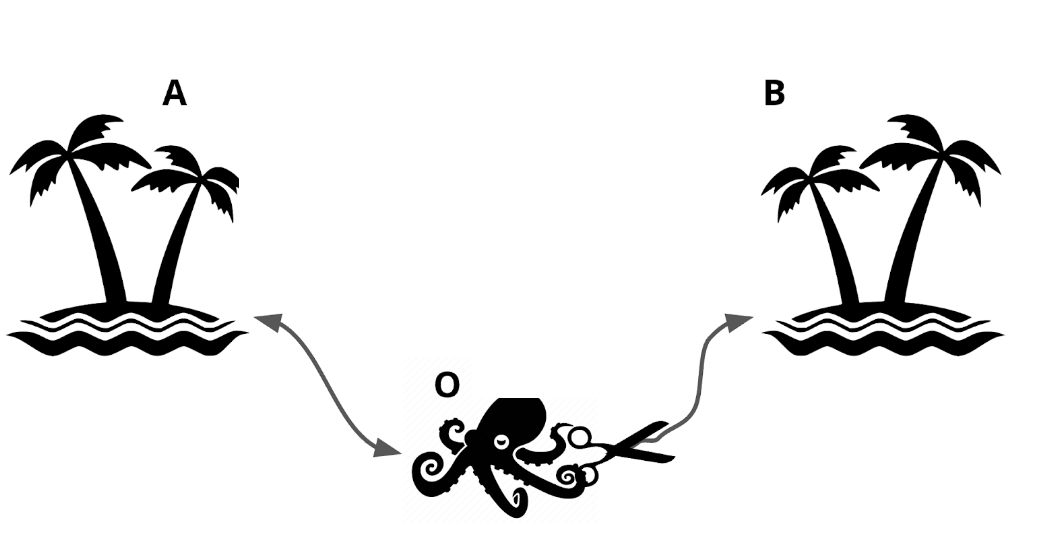
\includegraphics[scale=.20]{./images/octopusTest.png}
\caption[Soraya Boza.]{The octopus test. In the upper panel the octopus is
observing the information being passed back and forth. At a certain point the
octopus intercepts the wire and starts passing statistically similar messages
to the person on the first island. This is shown in the lower panel. The
communication is convincing, and the person on the left does not realize what
has happened (the poor person on the right is just out of luck at this point).
It has been argued that the octopus would not understand the information it
passed along, even if it was convincing to the human. Moreover, it has been
argued that the octopus would fail to produce convincing text in certain novel
situations.
}
\label{octopusTest}
\end{figure}


\subsection{LLMs and Behavioral Sciences}\label{llmsBehavioral}

% Generaly, how does this impact different approaches to linguistics:
% Chomskyan, Cognitive linguistics (Lakoff), etc? Eric T comment: The canonical
% type of example to use, that I think would be helpful, for why we are taking
% these dot products of influence across tokens, is a standard disambiguation
% example (e.g., `I went to the bank to cash my paycheck`, vs `We ate a picnic
% on the bank`). The transformer lets you come up with a new embedding that
% better represents the semantics of the tokens based on their context. The
% meaning of ‘bank’ just based on the original token embedding (say, from
% word2vec) is unclear but the self-attention step will allow meanings to
% propagate across tokens and push them in the right direction.   This point
% about context is in your chapter, but I worry it is getting lost a bit in all
% the technical details, so I think it  may deserve a bit more focus about how
% it's supposed to work. You can make this point even without mentioning
% key/value/query stuff or multiple heads (multiple heads is sort of a
% secondary or even tertiary point). The K/V/Q matrices add to this
% contextualization the power of tunable parameters (this is my admittedly
% limited understanding based partly on this really good video:
% https://www.youtube.com/watch?v=tIvKXrEDMhk ).

As noted above, BERT, an early transformer model, attracted interest from
linguists and psychologists. Despite being trained without any explicit
knowledge of grammar, it learned many aspects of syntax, including subject-verb
agreement, reflexive pronouns, and hierarchical sentence structure
\cite{goldberg2019assessing, linzen2021syntactic, tenney2019bert}. For example,
it has been shown that BERT's attention heads often focus on specific
linguistic roles, such as the direct objects of verbs or the determiners of
nouns \cite{clark2019does}. Some attention heads display broad attention across
entire sentences, while others are highly focused, suggesting a complex,
multi-faceted approach to language understanding within the model. This is
similar to earlier work on SRN's (see chapter
\extref{ch_supervised_recurrent}), but with the difference that much
longer-range dependencies in a stream could be captured
\cite{mcclelland2020placing}, thanks to attention heads which represent
pairwise relationships between all tokens in a context window. 

Chatbots powered by LLMs have become target ``subjects'' of a variety of
psychological experiments to assess the scope of their resemblance to humans.
We can take the same exact stimuli used for humans and use them for a chatbot.
In fact, some have argued that LLMs may be used as a substitute for human data
collection in future psychological research \cite{aher2023using,
dillion2023can}.

% The generalization (genuine intelligence) vs recall (stochastic parrot) debate
% discussed above generates testable predictions that are being studied in
% research labs. Generalization predicts that LLM responses should exhibit
% context dependence (such as word list composition effects in a
% psycholinguistic rating task), while recall predicts that LLM responses should
% not be sensitive to context. The generalization hypothesis makes predictions
% about what sorts of functions an LLM should be able to assemble, while the
% recall hypothesis predicts that LLMs should perform approximately equally well
% on tasks as long as the information is similarly present in its training data.
% For example, according to the generalization hypothesis, LLMs may be able to
% assemble functions that resemble human language use at the token level (such
% as word ratings) but should do poorly at approximating human reaction times in
% psycholinguistic studies because the dynamics that govern language production
% and comprehension at this timescale are abstracted over in token-level
% language data. The recall hypothesis, in contrast, would predict no difference
% in LLM performance across these two tasks because information about human
% performance on both of these metrics is equally available in its training data
% in the form of published studies.

Much of this work has related LLM behavior to known psycholinguistic effects.
For example, LLMs appear to reproduce human word rating norms on variables such
as  age of acquisition, arousal, concreteness, dominance, familiarity, gender
association, imageability, and valence \cite{trott2024augment,
kello2024emergent}. Humans and LLMs rated words across all of the categories in
a remarkably similar ways. Figure \ref{humanVsLLM} which shows these
correlations on a list of 390 words, with some correlations approaching .9,
which is very strong.  As an example, here is how valence is defined in such an
experiment:
\begin{quote}
a measure of value or worth. A word is NEGATIVE if it represents something
considered bad, whereas a word is POSITIVE if it represents something
considered good. Rate the valence of each of the following words on a
continuous scale from 1.0 (VERY NEGATIVE) to 9.0 (VERY POSITIVE), with the
midpoint representing NEUTRAL.
\end{quote}
Here are some examples of mean ratings on valence by humans and several LLMs,
for two words:

\begin{center}
\begin{minipage}{0.45\linewidth}
\begin{tabbing}
``affair'' \\
\hspace{1em}Human:\quad \= 2.438 \\
\hspace{1em}GPT-3.5:\> 3.98 \\
\hspace{1em}GPT-4:\> 4.05 \\
\hspace{1em}GPT-4o:\> 3.1 \\
\hspace{1em}Gemini1.5:\> 3.8
\end{tabbing}
\end{minipage}
\hspace{0.05\linewidth}
\begin{minipage}{0.45\linewidth}
\begin{tabbing}
``bead'' \\
\hspace{1em}Human:\quad \= 5.394 \\
\hspace{1em}GPT-3.5:\> 5.35 \\
\hspace{1em}GPT-4:\> 5.3 \\
\hspace{1em}GPT-4o:\> 5.38 \\
\hspace{1em}Gemini 1.5:\> 5.4
\end{tabbing}
\end{minipage}
\end{center}

\begin{figure}[ht]
\centering
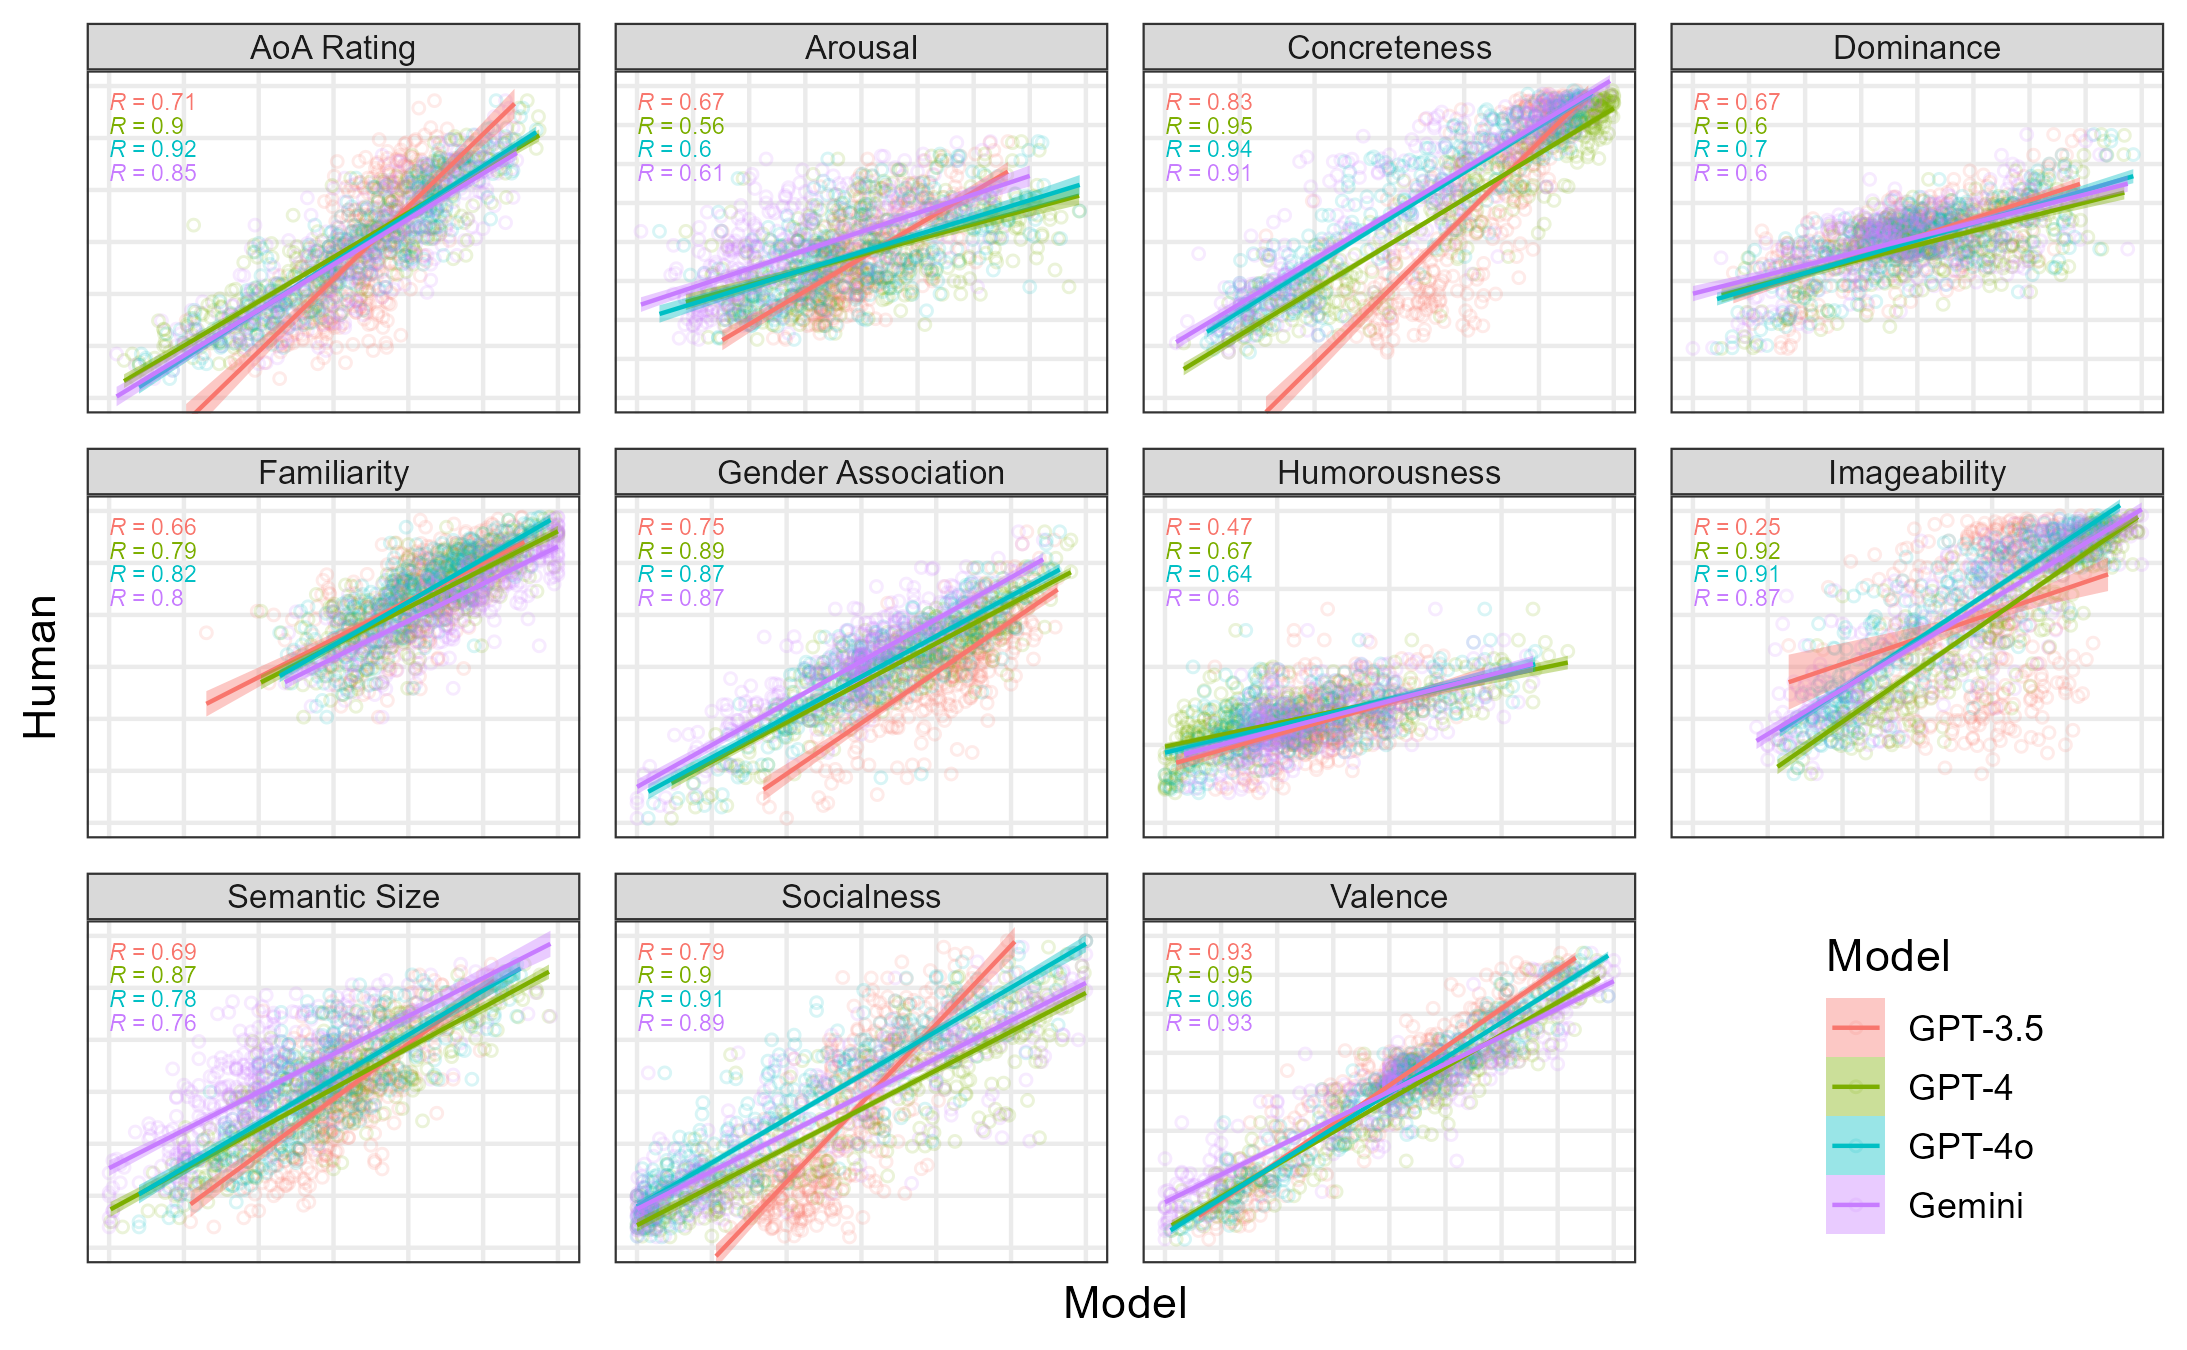
\includegraphics[scale=.8]{./images/humanVsLLM.png}
\caption[Figure borrowed from Kello et al. (2025, under review) with author
permission.]{Correlations of mean ratings  for 11 psycholinguistic variables
between LLMs ($x$-axis) and humans ($y$-axis) on a list of 390 words. Overall,
LLMs closely match human performance on word ratings across variables, with
some correlations reaching 0.9 or higher. Correlations are weakest for arousal,
dominance, and humorousness, which the authors argue is because these variables
are more ambiguous in meaning (consistent with greater variability in human
ratings, not shown). In later analyses, the authors show that the
correspondence between human and LLM ratings on these variables tracks human
inter-rater reliability: The more agreement in human ratings (i.e., lower
variability), the better LLMs are able to match human behavior. .}
\label{humanVsLLM}
\end{figure}

Additionally, Cai et al. (2023) reported that LLMs appear to mimic human
linguistic biases, such as sound-shape association (e.g., the ``kiki-bouba''
effect, in which arbitrary shapes are associated with specific nonsense words;
for example ``kiki'' is mapped to a more spikey structure and ``bouba'' to a
rounder one), sound-gender association (e.g., novel names ending in a vowel
compared to a consonant tend to be judged as more feminine sounding), semantic
and syntactic priming, and semantic illusion (e.g., noticing fewer errors in
sentences containing incongruous words when those words are semantically close
to congruous words), amongst others.

Some differences also emerge in this type of study.  For example, LLMs don't
seem to exhibit a preference for efficient language use, such as selecting the
shorter of two synonymous words (e.g., ``math'' versus ``mathematics'').
Similarly,  LLMs did not appear to resolve syntactic ambiguity in accordance
with efficient signal use, seen in humans. For example, humans have a tendency
to interpret ambiguous modifying expressions such as ``with the leash'' in
``walk the dog with the leash'' as identifying a type of dog rather than
describing an instrument for walking when multiple dogs are present. Modifying
expressions to resolve referential ambiguity (such as when there is more than
one dog that may be walked) is one property of efficient language use
\cite{frank2012predicting}. However, LLMs tested did not showed sensitivity to
the presence of referential ambiguity when interpreting syntactic ambiguity.
This discrepancy may indicate that LLMs are not currently governed by processes
related to the energy constraints that drive efficient cognitive solutions in
biological systems, which would offer a coherent difference between artificial
and natural intelligences.

LLMs have also been studied in relation to conceptual schemes in humans. Abdou
et al. show that language models can encode perceptual color relationships,
even though they have never ``seen'' colors the way sighted humans have (but
have only read about color relationship in texts) \cite{abdou2021can}. This
finding mirrors behavioral evidence that semantic judgments about color terms
are highly similar between congenitally blind and sighted individuals
\cite{marmor1978age, saysani2018colour}. Indeed, blind individuals have been
shown to possess rich visual knowledge, indicating that some aspects of
'embodied' experiences are available in the structure and use of language
\cite{kim2019knowledge, liu2025learning}. Liétard et al. find that LLMs can
predict relative geographic distances between cities \cite{lietard2021do}.
Christiansen et al. report that LLMs organize concepts in ways that correlate
with human conceptual structures \cite{christiansen2023large}. These findings
collectively suggest that LLM representations are not ``empty symbols'' as in
traditional computer programs (see the discussion in
\extref{classicalAIComparison}). Instead, they are content-rich and structured
similarly to human mental representations.

Finally we note a lively debate about the extent to which LLMs are capable of
reasoning. Melanie Mitchell studied early transformer architectures (and deep
nets before them) and argued that they are not as intelligent as they appear,
in light of their tendency to fail at reasoning tasks, especially those that
require generalization and transfer of knowledge (compare the discussion of
stochastic parrots and the octopus test above).  An example that went viral
around 2023 was asking LLMs to  ``count the number of Rs in 'strawberry'''.  At
the time, they often failed at such purely symbolic tasks.  Mitchell,
discussing these failures, concluded that ``Giving machines common sense will
require imbuing them with the very basic `core,' perhaps innate, knowledge that
human infants possess about space, time, causality, and the nature of inanimate
objects and other living agents, the ability to abstract from particulars to
general concepts, and to make analogies from prior experience. No one yet knows
how to capture such knowledge or abilities in machines'' \cite{mitchell2021ai}. 

Subsequently transformer based architectures like GTP-4 performed at high
levels in standardized tests like the LSAT, the SAT, and the Bar (though not
quite as well at writing). See figure \ref{llmStandardExams}. Multiple studies
also showed that LLMs could perform as well as or better than humans on
analogical problems, including problems developed by Mitchell herself
\cite{webb2023emergent}.  Mitchell has responded, noting  that transformers
perform well on simple analogies but that performance declines sharply on  more
complex analogies \cite{lewis2025evaluating}. The topic remains hot as of 2025.
In June 2025 a group at Apple published a paper whose title begins with``The
Illusion of Thinking'' \cite{shojaee2025illusion}, which claims that large
reasoning modelings like LLMs `` face a complete accuracy collapse beyond
certain complexities''. The charge was met days later by a post by Anthropic
called ``The illusion of the illusion of thinking" \cite{opus2025illusion},
which claimed that the Apple group's work ``primarily reflect experimental
design limitations rather than fundamental reasoning failures'' and that when
controlling for these errors that LLMs can succeed on reasoning tasks reported
as failures in \cite{shojaee2025illusion}. So the issue is hot and ongoing.

\begin{figure}[ht]
\centering
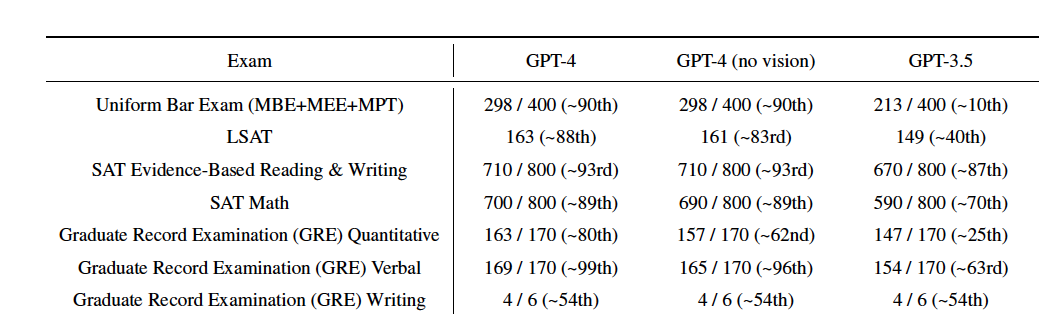
\includegraphics[scale=.8]{./images/llmStandardizedExams.png}
\caption[From \cite{achiam2023gpt}.]{Some of the performance results on
standardized tests noted in the GPT-4 technical report.  Note the high
performance on most tests shown, but middling performance on the Writing GRE.
}
\label{llmStandardExams}
\end{figure}

\begin{figure}[ht]
\centering
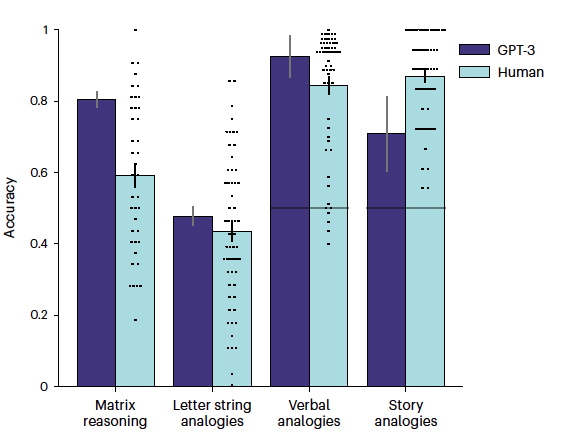
\includegraphics[scale=.8]{./images/llmAnalogical.png}
\caption[From \cite{webb2023emergent}.]{LLMs perform comparably to humans on a
variety of analogical reasoning tasks. The Letter problems are based on
problems developed by Hofstadter and Mitchell.
}
\label{llmAnalogy}
\end{figure}

% From apple paper: In this work, we systematically investigate these gaps with
% the help of controllable puzzle environments that allow precise manipulation
% of compositional complexity while maintaining consistent logical structures.
% This setup enables the analysis of not only final answers but also the
% internal reasoning traces, offering insights into how LRMs “think”. Through
% extensive experimentation across diverse puzzles, we show that frontier LRMs
% face a complete accuracy collapse beyond certain complexities. Moreover, they
% exhibit a counter-intuitive scaling limit: their reasoning effort increases
% with problem complexity up to a point, then declines despite having an
% adequate token budget. By comparing LRMs with their standard LLM counterparts
% under equivalent inference compute, we identify three performance regimes:
% (1) low- complexity tasks where standard models surprisingly outperform LRMs,
% (2) medium-complexity tasks where additional thinking in LRMs demonstrates
% advantage, and (3) high-complexity tasks where both models experience
% complete collapse.

% https://www.nature.com/articles/s41562-023-01659-w Also something multimodal

\subsection{LLMs and Neuroscience}

We have seen in earlier sections that neuroscientists have used convolutional
neural networks (CNNs) to predict brain activity (section
\extref{cnn_applications}). In a similar way, researchers are now leveraging
transformer-LLMs to understand how our brains process language. 

For example, several groups \cite{pasquiou2022neural, schrimpf2021neural,
caucheteux2022brains} have explored the relationship between internal
activation patterns in LLMs as they process a text and patterns of human brain
activity elicited by the same  human beings when they process the same text.
The approach taken is generally this:  
\begin{enumerate}
  \item A text (such as \emph{The Little Prince}) is selected.
  \item The text is fed into an LLM.
  \item The LLM's internal activations are recorded and time-locked to each
  token (word or punctuation mark) in the text.
  \item A human subject reads or listens to the same text while their brain
  activity is recorded using EEG, MEG, or fMRI.
  \item The brain activity is  aligned (time-locked) to the same tokens.
  \item A linear model is trained to predict the human brain responses from the
  LLM activations.
  \item The model is tested on held-out data (e.g., new passages of text) to
  assess how well the LLM-derived features predict neural activity. That is,
  given a new text, can the LLM predict what will occur in some part of the
  human brain?
\end{enumerate}

Because this procedure can be applied across different layers of LLM and
different brain regions, it can be used to produce  a set of prediction scores
indicating which parts of the model correspond best to which areas of the
brain. These results effectively map layers or the LLM to the brain's language
network.

Transformers often outperform other computational models in predicting brain
activity---a result echoing earlier work showing that deep CNNs predict
activity in the visual system with higher accuracy than prior theoretical
models of the visual system do (section \extref{cnn_applications}). Some
studies suggest that even untrained models can predict neural activity
moderately well, suggesting that the \emph{architecture itself} captures
aspects of linguistic processing, though performance improves substantially
with training. ``For example, across the three datasets, untrained GPT2-xl
achieves an average predictivity of $\sim$ 51\%, only $\sim$ 20\% lower than
the trained network. A similar trend is observed across models: Training
generally improves brain scores, on average by 53\%''
\cite{schrimpf2021neural}. Figure \ref{brainPredictionLLM} shows some of the
areas where activity is most strongly predicted by LLMs.

\begin{figure}[ht]
\centering
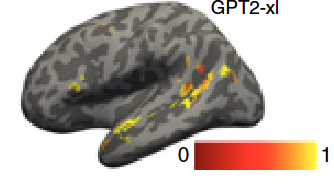
\includegraphics[scale=.9]{./images/brainPredictionsLLM.png}
\caption[From \cite{schrimpf2021neural}.]{Highlighted regions correspond to
areas whose brain activity (voxel activity in fMRI) that are best predicted by
the internal activation patterns of an LLM.
}
\label{brainPredictionLLM}
\end{figure}

Prediction tends to be strongest for activations in the middle layers of LLMS
\cite{caucheteux2022brains}, but the details remain unclear (see
\cite{schrimpf2021neural}, figure 2C), and this work will probably be best
pursued along side work in mechanistic interpretability  (chapter
\extref{ch_mechinterp}), where studies suggest that attention heads located
early in the model's forward pass tend to deal with syntactic features,
composing these into semantic features in the middle of the forward pass, and
finally refocusing on syntax at the end of the pass.

% Word-by-word surprisal values generated by BERT correlate with human reading
% times and EEG responses (heilbron2022distinct, A hierarchy of linguistic
% predictions during natural language comprehension) indicating that such
% models capture not only neural responses but also moment-to-moment processing
% difficulty experienced during language comprehension.

\subsection{LLMs and Philosophy}\label{llmPhilosophy}

LLMs have had a wide-ranging and ongoing impact on philosophical discussions of
AI, given that they have done many of the things long-time AI skeptics doubted
would ever be possible in a machine, like speak fluent language and arguably
pass the Turing Test.\footnote{An extensive and helpful review of philosophical
issues through 2024 is \cite{milliere2024philosophical1,
milliere2024philosophical2}. Multiple new papers on topics relating to AI
appear each week at \url{philPapers.org} so the areas is quite active.} That
this was done by a neural networks has been seen by many as a decisive win for
connectionism relative to the old debate about whether neural networks or
symbolic architectures are best-suited to modeling cognition (see section
\extref{cog_rev}), but that has not settled the issue. We here review  a
smattering of topics to give a sense of the debates most relevant to the topic
of the book: neural networks and cognitive science.  

% Other questions: Turing Test, are they conscious, do they have world models,
% and AI ethics

First, there is an old debate about whether passing the Turing Test sufficient
to conclude that a system really understands anything. Doubts about the ability
of machines to understand language have a long history, and there is a whole
class of arguments to the effect that a system can't understand the meanings of
words just by manipulating symbols, or by transmitting information. These are
sometimes called \emph{unusual realization arguments}, given that these
arguments
\begin{quote}
ask us to imagine people carrying out simple operations on bit streams,
connectionist-like computations on activations patterns, or the control
operations of the central processing unit of a computer. For example, Dneprov
asks us to imagine a stadium full of people who pass 0's and 1's to one another
on the basis of instructions announced over a loudspeaker. We can further
imagine that this stadium is linked to an input-output device that enables it
to pass the Turing Test. We can then ask ourselves: do we really think this
stadium full of people has consciousness or genuine understanding?
\cite{noelle2022artificial}
\end{quote}

Some have argued (often based on the ``stochastic parrot'' intuitions canvassed
above) that these arguments apply to LLMs. They can pass the Turing Test by
manipulating information in a clever way--here based on a statistical
aggregation of the internet--but they don't truly understand anything, and they
are certainly not conscious \cite{hamid2023chatgpt}. In fact, some LLMs have
themselves claimed that the Chinese Room argument (a famous form of the unusual
realization argument) applies to them \cite{sep-chinese-room}! 

However, others argue that LLMs do understand the meaning of the words they
produce. Relying on findings presented above, Sogaard
\cite{sogaard2023grounding} argues that the representations LLMs use are
grounded (that is, are meaningful) in virtue of their alignment with human
neural, cognitive, and perceptual spaces. These are not like the empty symbols
passed along in Dneprov's stadium or in other ``unusual realization
arguments.'' Here, the LLM manipulates representations that have internal
structures aligned with those of the human mind.\footnote{A philosophical
argument that LLMs could, with some additions relating to agency, produce
genuine understanding, is in \cite{borg2025llms}.} 

Another long-standing argument against machine intelligence due to Hubert
Dreyfus \cite{dreyfus1992computers} is that no computer or neural network could
ever have truly human capacities, because they were not raised in the real
world and can only parrot back what they were programmed or trained to say, at
best with moderate abilities to generalize beyond that (Bender and Keller's
argument develop this idea with respect to LLMs and argue these considerations
are why the octopus would pass the test). However, humans with their embodied
human existence develop an intuitive sense of the full context of the lived
world. To show this, one of the authors (Yoshimi), who has regularly taught
Dreyfus'  argument for many years, would have the class ask strange or unusual
questions to AI systems and chatbots of earlier years, like ``What would happen
if a penguin were to juggle alligators." The systems invariably struggled to
say anything meaningful (though some chatbots did pretty well using tricks,
like pretending to be a teenager saying ``lol who cares''). But current
iterations of LLMs like ChatGPT do just fine with such questions, suggesting
that the old problem of background knowledge may have been resolved. 

The recent success of LLMs in producing coherent and intelligent-seeming
linguistic behavior has also revived the old debate about whether neural
networks or symbolic architectures are best-suited to modeling cognition (see
section \extref{cog_rev} as well as \cite{king2024large}). In 2023 Noam Chomsky
(representing the symbolic approach) wrote a New York Times guest essay titled
``The False Promise of ChatGPT'' in which he claimed that statistical
approaches to language like neural networks ``will degrade our science and
debase our ethics by incorporating into our technology a fundamentally flawed
conception of language and knowledge'' \cite{chomsky2023noam}. The essay echoes
many decades of research on his part arguing against statistical learning
theory and behaviorist or empiricists approaches to language. 

The old debate went something like this. According to the symbolic approach,
stimuli activate symbols which can be re-arranged and composed in arbitrary
ways, in accordance with innate rules (like the rules of grammar). This innate
capacity for combination and recombination is what gives human beings their
vast, indefinite expressive power. Neural networks only learn statistical
associations, and are thus brittle. They cannot combine and recombine symbols
to produce arbitrary responses to queries and to think in arbitrarily complex
ways. As Chomsky says, echoing the stochastic parrot and octopus arguments,
Chat GPT is ``a lumbering statistical engine for pattern matching, gorging on
hundreds of terabytes of data and extrapolating the most likely conversational
response or most probable answer to a scientific question.''
% Citations above

% Lupyan below and links; https://arxiv.org/abs/2506.01820
The immediate response from a neural network enthusiast will be to simply point
to the ability of LLMs to answer questions in arbitrary ways. It seems like an
existence proof against the old symbolic AI arguments: we have a system based
on statistics that does what supporters of the symbolic approach claim it
cannot do. More principled responses look to the internal structure of these
systems and how they work. Some have noted that systems based on word
embeddings can in fact produce the kinds of compositional patterns emphasized
in symbolic AI. Much of this work is now being carried out in the field of
mechanistic interpretability (chapter \extref{ch_mechinterp}). 

% Chomsky 1980 cite. Also cite Gary Marcus Perhaps "inductive bias" is the way
% to fix it. Iris discussed it. 
A natural response from the classical symbolic perspective is to note that
humans learn a language based on a relatively limited input stream. Toddlers
can talk pretty well based on  far less data than a trained LLM is exposed to.
The fact that humans can learn language based on limited input data is
sometimes used as a ``poverty of the stimulus'' argument against the kind of
empiricist approach assumed by an LLM.  LLMs are not trained the way humans
are; they must be trained on the entire internet--``gorging on hundreds of
terabytes of data''.  This is not at all realistic. Some have begun to pursue
these arguments systematically, and suggested that when language models
\emph{are} trained on naturalistically realistic data, they are limited in the
ways Chomsky and others predicted they should be \cite{lan2024large}.

Finally, another response is to say that neural networks are in fact processing
language symbolically. If mechanistic interpretability succeeds, it will have
succeeded in finding what the classical approach said would be there all along:
a  symbolic system, reading and writing representations to the residual stream.
We are not yet aware of someone making this argument in print, but it's just a
matter of time.\footnote{Consider these quotes from
\cite{elhage2021mathematical}: ``Both the attention and MLP layers each
``read'' their input from the residual stream (by performing a linear
projection), and then ``writ'' their result to the residual stream by adding a
linear projection back in... We generally think of the residual stream as a
communication channel, since it doesn't do any processing itself and all layers
communicate through it... some MLP neurons and attention heads may perform a
kind of ``memory management'' role, clearing residual stream dimensions set by
other layers by reading in information and writing out the negative version...
The fundamental action of attention heads is moving information. They read
information from the residual stream of one token, and write it to the residual
stream of another token.''}

Across these examples, much of the real nitty gritty concerns what is going on
inside the guts of an LLM. Clearly they are doing something more intelligent
than consulting a giant lookup table.\footnote{This idea relates to another old
thought experiment in philsophy of cognitive science, the ``blockhead example''
(due to Ned Block), according to which a system that behaved intelligently just
by consulting such a table would not actually be considered intelligent
\cite{milliere2024philosophical1}.} So what \emph{is} going inside an LLM? Are
the symbols grounded? Is there a world model in there? Is a compositional
symbol system lurking?  We hope we have provided some guidance to thinking
about what happens in the guts of these machines with all the explanations and
visualizations (and pointers to other tools and visualizations) in this
chapter, and we also note that the topic is itself being actively pursued in
the area of mechanistic interpretability, discussed in chapter
\extref{ch_mechinterp}. 
% of course circuits promote generalization, but it feels different Millier,
% part 2:  "The entire phenomenon is thus not a sudden onset of generalization
% ability, but rather a gradual amplification of structured mechanisms encoded
% in the weights, followed by pruning of unnecessary components. Importantly,
% these findings speak against the skeptical view of LLMs discussed in Part I
% (Millière & Buckner 2024), according to which they are analogous to giant
% lookup tables with memorized input-output pairs. While the initial training
% phase does support that view, subsequent phase transitions show that
% Transformer models are perfectly capable to learn general, rule-like
% algorithms to solve tasks, including tasks as rigid and well-defined as
% arithmetic problems."

% Mitchell (2025) skeptical about emergence in LLMs:
% https://arxiv.org/pdf/2506.11135



\section{LLMs in Practice}\label{transformersInPractice}

This final section discusses things you need to know to actually use an LLM in
a functional system in a technical stack (a collection of components and
technologies used together in a working production system).  It's one thing to
know what an LLM is in terms of matrices, etc.  But it is a separate thing to
know how to integrate an LLM into a running system that people can interact
with.  There are many practical matters to address.

Even though these are practical issues that have emerged around building
effective LLMs, with virtually no thought given to cognitive science, we've
seen that historically it is not uncommon for engineering tools to end up being
relevant to cognitive science. That trend continues here. Thought there is
little discussion of it yet, all of the topics discussed here are relevant to
cognitive science and to understanding how minds work. 

\subsection{Pre-Training, Post-Training, and Fine-Tuning}

Most LLMs are built on top of \glossary{foundation models} that have been
pre-trained on vast amounts of data, some subset of the entire internet (see
section \ref{internetese}). This pre-training gives them broad linguistic
competence and general background knowledge, arguably solving the problem of
``background knowledge'' (section \ref{llmPhilosophy}). However, to adapt a
model for a specific domain--for example, to build a system that can analyze a
set of legal documents--it must be fine-tuned on a smaller, targeted corpus.
% The pre in pre-training is I think relative to fine-tuning which is the
% "post" part

\glossary{Fine-tuning} involves additional training with a relatively small
learning rate, slightly nudging the weights to better capture the new domain.
This can be expensive and computationally heavy if done across the entire
model, but that are various technical tricks that make this more
efficient.\footnote{For example, LoRA (Low-Rank Adaptation), which adds a small
number of trainable weights so that only a subset of parameters changes. This
can be viewed as biasing the model toward a particular task without fully
rewriting its knowledge. Models like DeepSeek have used techniques like LoRA in
combination with curated data cleanup to good effect.} A gripping example of
fine-tuning is the case of the late singer Lou Reed's wife creating a special
LLM which was fine-tuned using ``a vast cache of Reed's writing, songs and
interviews'', giving it a bit of his
personalty.\footnote{\url{https://tinyurl.com/yyd2hjh5}.}  Many fine-tuned
foundaton models now exist, in biomedical, legal, and many other domains.
% References

One notable and familiar form of fine-tuning is all the techniques of
``instruction tuning'' or ``alignment tuning'' like reinforcement learning with
human feedback.  These processes are fine-tuning techniques that give LLMs
their familiar personalities, and are discussed further in the chapter on value
alignment. They help it know when to stop talking (the ``when-to-shut-up
circuit'') but they also smooth out the model's personalty. We discuss the
post-training pipeline more extensively in \extref{ch_value_alignment}.
% TODO: Add link to that chapter when we have it. Lupyan notes, esp on what
% GPT3 was like and the role of fine tuning Reference back to Elman and staged
% learning.  Also the Cowan and activated long term working memory Intuitive
% idea of things you know deeply in your bones from way back vs more recently
% learned

\subsection{Prompt Engineering} 

We already saw that in-context learning is like reasoning in working memory,
which can be contrasted with training the billions of parameters of a model,
either initially when training a foundation model or later in fine-tuning.

There is another approach to processing in a transformer model that is not
quite a form of learning, but that still impacts its ability to process
information.  That is, by manipulating the text that flows through the
transformer, using the ``recursive trick'' described in section
\ref{recursiveTrick}.  We don't just turn on the network cold and have it start
processing information.  Suppose you enter a  query into a transformer like
ChatGPT. This is  often called a \glossary{user prompt}, the thing you ask the
system about. However, that  not what is actually fed to the network. Behind
the scenes other information is added.  At the very start of the query a whole
block of text called the \glossary{system prompt} is pre-pended. It might look
something like this

\begin{quote}
You are a helpful, honest, and friendly assistant.\\
You answer clearly and politely.\\
If you don't know something, say so.\\
Do not make things up.
\end{quote}

This sets the whole tone of a conversation. 

So when you query the system ``Tell me about the history of Bulgaria'' what is
actually sent in to the neural network is the whole system prompt plus your
user prompt.\footnote{As well as other information that distinguishes you from
the system. Much of this is hidden. The mechanics of this is handled via
special tokens and other structures. For a sense of how this works search
``chatml'', which is ChatGPT's markup language.}
% User prompts can ``prime'' the model to act in particular ways, even
% overriding system-level instructions (as seen in jailbreaks).

But the idea does not end there. Depending on what you say in your prompt,
other extra information can be added, some of it behind-the-scenes and
invisible to the user, and much of it conditional on what you ask. That is, a
system (external to the neural network) can detect the nature of the prompt and
dynamically add extra instructions into the prompt before sending it to the
model. This is encoded in a \glossary{prompting strategy}. For example, if you
ask a mathematics question, behind the scenes it might add this to your query:
``When answering math questions, show all steps and use LaTeX formatting.''
% Prompt injection. Prompt orchestration.  What are the right terms here? There
% are lightweight and heavyweight forms of prompt adjustment. Simply rewriting
% your input is one way; using tools like LangChain to programmatically slot in
% user queries, context, and examples is a more structured approach. This has
% led to the emergence of ``LLM orchestration,'' which involves managing not
% just the prompt itself but the whole lifecycle of interaction—storing memory
% between sessions, structuring context, and choosing what background
% information to include.

% Reference
In fact, this kind of strategy is behind what has been called the ``reasoning
revolution'' in LLMs, which began around 2023. Earlier LLMs had serious trouble
with reasoning tasks, as emphasized in critiques like those of Melanie Mitchell
(see section \ref{llmsBehavioral}). However, simply by a special form of prompt
injection, the systems can do much better.  For example, \glossary{chain of
thought} encourages the model to articulate intermediate reasoning steps, which
often improves its final answer. This was evident in the example above of
telling the system to ``show all steps''. In this way, as the model is working
through a problem, it feeds itself information, into its ``working memory'',
that it can allow it to answer things.

This is very close to an old idea in embodied cognition that we don't solve
problems on our own, but only do so in the context of environental artifacts.
To take a classic example from the PDP volumes, when solving a long division
problem it is essential to have a piece of paper available where intermediate
results are written down. Without pane and paper could you compute 21 divided
by 4.2? The paper is used to store intermediate results. It's not a special
brain circuit, it's a way of using environmental artifacts to help in a
computation. In a similar way the LLMs is spitting out results that then get
fed back to it.

% Bring out more of the  connection between framing and embodied cognition, and
% how we can’t put everything in our minds at once and so we need to work
% closely with external artifacts, often making a to-do list or breaking a
% prompt down in the subparts or talking to someone and having a debate as in
% debate based reasoning so there’s a lot of cognitive significance here it’s
% not just about the brain. It’s about how the brain and artifacts interact.
% Can ask gpt for examples.  For example how you ask a question 

These days quite a bit of this happens, and you can see it on systems like
ChatGPT when it flashes information about what its thinking about.
 
% Multi-hop reasoning https://arxiv.org/abs/2403.09629 "Chain of Thought" it
% prompts itself

\subsection{Agentic Systems}

% David: you said keywords here are "wrapper" and "scaffold."

A final trend to note is the advent of \glossary{agentic systems}, wherein an
LLM delegates subtasks to external software or to other LLM instances. The idea
is that an LLM does not just churn out a text response, but is rather empowered
to\emph{do} things, like an agent. It can, for example send a query to the
internet. The result of this query can then be fed back into the LLM, and it
can then make a more informed response that reflects information from after its
training cutoff date. By this point this is probably familiar to you. LLMs will
routinely query the internet (modern system give you a sense that are doing
this, flashing an image of the websites they are querying). Note that the
transformer is still ultimately generating text out. It's just that we don't
necessarily have to understand that text output as natural language; text
prediction is just as expressive as keyboard input, and so transformers can be
equipped to write and run code, browse the internet, jot down persistent notes,
etc.

Note that a special model does not necessarily have to be fine-tuned for this
to work. Indeed, agentic systems today are generally general-purpose frontier
LLMs, just set up with an appropriate system prompt and placed inside a
software wrapper that will take the model's written source code (or whatever
special text it is outputting) and respond to that output accordingly. It is
the \emph{LLM} that is doing all the heavy-lifting here; if the transformer
were unable to write Python, or unable to leave coherent notes to itself, etc.,
then no toolset would fix that deficiency. What we are doing with agentic
wrappers is just giving the model tools that is either already knows how to use
or is able to learn to use in-context. To the extent that models beat Pokemon,
write novel code, etc., it is a glimmer of their general competence with
arbitrary tools and interfaces shining through.

LLM software engineers in particular are now commmonplace in computer
programming, in IDEs like Cursor. A user can ask for a particular function,
described in natural language, and the AI will generate the function and debug
its code as runtime errors appear.

This is obviously much closer to actual agentic behavior than the pure chat
model, and so the relevance to cognitive science should be obvious.

% Society of mind Ron Sun: https://arxiv.org/abs/2410.20037 Mixture of Experts 

% Rags. Semantically encode a document. (ref to that chapter) Finds similar
% things from your corpus. Fills those semantically similar things into anther
% slot. So rather than filing up a giant context window, can selectively sample
% from it and the RAG will fill that.
% https://en.wikipedia.org/wiki/Retrieval-augmented_generation. Do a semantic
% encoding of your entire corpus. everything you want it to reference. Like a
% library of pdfs. Run a prelim system that goes through a datbase of pdfs and
% codes up each chunk in terms of what it's about. Then when you load your
% model it fits within a context window all the information that is as close as
% possible to your query. A way to fill the context window with relevant
% material when your overall corpus is too big to fit in the context menu. 

% See Millier part 2, 3.1.2. ‘Agent’ systems
% https://developers.googleblog.com/en/agent-development-kit-easy-to-build-multi-agent-applications/
% You can see this working in claude 2.7. Shows itself writing the code to call
% out to a console log what's in that document on the internet. LLM takes the
% task, breaks it up and sends bit of the task to different agents. LLM is
% instructed to take your task, decompose it, and pass those to different
% agents. Tim has a cool example of a simulated hospital:
% https://arxiv.org/html/2405.02957v3 The relevance here is to the old cogsci
% debates of merging AI and Connectionism.
